\documentclass[journal=asbcd6,manuscript=article]{achemso}

\usepackage{natbib}
\usepackage{setspace}
\usepackage{xkeyval}
\usepackage{array}
\usepackage{listings}
\usepackage{lmodern}
\usepackage{mathpazo}
\usepackage{geometry}
\usepackage{microtype}
\usepackage{url}  % Formatting web addresses
\usepackage{ifthen}  % Conditional
\usepackage{multicol}   %Columns
\usepackage[utf8]{inputenc} %unicode support
\usepackage{amsmath}
\usepackage{amssymb}
\usepackage{mathtools}
\usepackage{epsfig}
\usepackage{epstopdf}
\usepackage{graphicx}
\usepackage{textcomp}
\usepackage{multirow}
\usepackage{booktabs}
\usepackage{natmove}
\usepackage{float}
\usepackage[margin=0.1pt,font=footnotesize,labelfont=bf]{caption}
\usepackage[version=3]{mhchem} % Formula subscripts using \ce{}
\usepackage[T1]{fontenc}       % Use modern font encodings
%\usepackage[square,sort,comma,numbers,sort&compress]{natbib}
%%%%%%%%%%%%%%%%%%%%%%%%%%%%%%%%%%%%%%%%%%%%%%%%%%%%%%%%%%%%%%%%%%%%%
%% If issues arise when submitting your manuscript, you may want to
%% un-comment the next line.  This provides information on the
%% version of every file you have used.
%%%%%%%%%%%%%%%%%%%%%%%%%%%%%%%%%%%%%%%%%%%%%%%%%%%%%%%%%%%%%%%%%%%%%
%%\listfiles

%\bibliographystyle{achemso}
\newcommand*\mycommand[1]{\texttt{\emph{#1}}}
%%%%%%%%%%%%%%%%%%%%%%%%%%%%%%%%%%%%%%%%%%%%%%%%%%%%%%%%%%%%%%%%%%%%%

%%%%%%%%%%%%%%%%%%%%%%%%%%%%%%%%%%%%%%%%%%%%%%%%%%%%%%%%%%%%%%%%%%%%%
\author{Michael Vilkhovoy}
\affiliation[Cornell University]
{Robert Frederick Smith School of Chemical and Biomolecular Engineering, Cornell University, Ithaca, NY 14853}
\author{Nicholas Horvath}
\affiliation[Cornell University]
{Robert Frederick Smith School of Chemical and Biomolecular Engineering, Cornell University, Ithaca, NY 14853}
\author{Che-Hsiao Shih}
\affiliation[Purdue University]
{Davidson School of Chemical Engineering, Purdue University, West Lafayette, IN 47907}
\author{Joseph Wayman}
\affiliation[Cornell University]
{Robert Frederick Smith School of Chemical and Biomolecular Engineering, Cornell University, Ithaca, NY 14853}
\author{Kara Calhoun}
\affiliation[Stanford University]
{School of Chemical Engineering, Stanford University, Stanford, CA 94305}
\author{James Swartz}
\affiliation[Stanford University]
{School of Chemical Engineering, Stanford University, Stanford, CA 94305}
\author{Jeffrey D. Varner}
\email{jdv27@cornell.edu}
\phone{+1~(607)~255-4258}
\fax{+1~(607)~255-9166}
\affiliation[Cornell University]
{Robert Frederick Smith School of Chemical and Biomolecular Engineering, Cornell University, Ithaca, NY 14853}
%%%%%%%%%%%%%%%%%%%%%%%%%%%%%%%%%%%%%%%%%%%%%%%%%%%%%%%%%%%%%%%%%%%%%
\title{Sequence Specific Modeling of \emph{E.~coli} Cell-Free Protein Synthesis}
%\abbreviations{MV,NH,JDV}
\keywords{Synthetic biology, constraint based modeling, cell-free protein synthesis}

\begin{document}

%%%%%%%%%%%%%%%%%%%%%%%%%%%%%%%%%%%%%%%%%%%%%%%%%%%%%%%%%%%%%%%%%%%%%
%% The abstract environment will automatically gobble the contents
%% if an abstract is not used by the target journal.
%%%%%%%%%%%%%%%%%%%%%%%%%%%%%%%%%%%%%%%%%%%%%%%%%%%%%%%%%%%%%%%%%%%%%
\begin{abstract}
Cell-free protein synthesis (CFPS) has become a widely used research tool in systems and synthetic biology.
In this study, we used sequence specific constraint based modeling to evaluate the performance of an \emph{E.~coli} cell-free protein synthesis system.
A core \emph{E.~coli} metabolic model, describing glycolysis, the pentose phosphate pathway, energy metabolism, amino acid biosynthesis and degradation was augmented with sequence specific descriptions of transcription and translation with effective models of promoter function.
Thus, sequence specific constraint based modeling explicitly couples transcription and translation processes and the regulation of gene expression with the availability of metabolic resources.
We tested this approach by simulating the expression of two model proteins: chloramphenicol acetyltransferase and dual emission green fluorescent protein, for which we have training data sets; we then expanded the simulations to a range of therapeutically relevant proteins.
Protein expression simulations were consistent with measurements for a variety of cases.
We compared the theoretical optimal solutions with an experimentally constrained case which suggested CFPS retained a growth-like operational memory that led to overconsumption of glucose, and low energy efficiency due to suboptimal oxidative phosphorylation activity.
Further, global sensitivity analysis identified the key metabolic processes that controlled the productivity, energy efficiency, and carbon yield of the process.
Taken together, sequence specific constraint based modeling offers a novel means to \emph{a~priori} estimate the performance of cell-free synthetic circuits.
\end{abstract}

% A sufficient energy supply with oxidative phosphorylation is instrumental for high energy efficiency and carbon yields; in addition, the translation rate could be optimized for higher productivity.

%%%%%%%%%%%%%%%%%%%%%%%%%%%%%%%%%%%%%%%%%%%%%%%%%%%%%%%%%%%%%%%%%%%%%
%% Start the main part of the manuscript here.
%%%%%%%%%%%%%%%%%%%%%%%%%%%%%%%%%%%%%%%%%%%%%%%%%%%%%%%%%%%%%%%%%%%%%

\section{Introduction}
Cell-free protein expression has become a widely used research tool in systems and synthetic biology, and a promising technology for personalized protein production.
Cell-free systems offer many advantages for the study, manipulation and modeling of metabolism compared to \textit{in vivo} processes.
Central amongst these is direct access to metabolites and the biosynthetic machinery without the interference of a cell wall or the complications associated with cell growth.
This allows interrogation of the chemical environment while the biosynthetic machinery is operating, potentially at a fine time resolution.
Cell-free protein synthesis (CFPS) systems are arguably the most prominent examples of cell-free systems used today \cite{Jewett:2008aa}.
However, CFPS is not new; CFPS in crude \textit{E.~coli} extracts has been used since the 1960s to explore fundamental biological mechanisms \cite{MATTHAEI:1961aa,NIRENBERG:1961aa}.
Today, cell-free systems are used in a variety of applications ranging from therapeutic protein production \cite{Lu:2014aa} to synthetic biology \cite{Hodgman:2012aa}.
However, if CFPS is to become a mainstream technology for advanced applications such as point of care manufacturing \cite{Pardee:2016aa}, we must first understand the performance limits and costs of these systems \cite{Jewett:2008aa}.
One tool to address these questions is constraint based modeling.

% Interestingly, many of the challenges confronting \textit{in~vivo} genome scale kinetic modeling can potentially be overcome in a cell-free system.
% For example, there is no complex transcriptional regulation to consider, transient metabolic measurements are easier to obtain, and we no longer have to consider cell growth.
% Thus, cell-free operation holds several significant advantages for model development, identification and validation.
% Theoretically, genome scale cell-free kinetic models may be possible for industrially important organisms, such as \textit{E.~coli} or \textit{B. subtilis}, if a simple, tractable framework for integrating allosteric regulation with enzyme kinetics can be formulated.
% Traditionally, stoichiometric models have also neglected explicit descriptions of metabolic regulation and control mechanisms, instead opting to describe the choice of pathways by prescribing an objective function on metabolism. Interestingly, similar to early cybernetic models, the most common metabolic objective function has been the optimization of biomass formation \cite{2002_ibarra_edwards_palsson_Nat}, although other metabolic objectives have also been estimated \cite{2007_schuetz_sauer_MolSysBio}.
% Recent advances in constraint based modeling have overcome the early shortcomings of the platform, including capturing metabolic regulation and control \cite{2013_hyduke_lewis_palsson_MolBioSys}. Thus, modern constraint based approaches are extremely useful for the discovery of metabolic engineering strategies and represent the state of the art in metabolic modeling \cite{2013_mccloskey_palsson_feist_MolSysBio, 2012_zomorrodi_maranas_MetaEng}.

Stoichiometric reconstructions of microbial metabolism, popularized by constraint based approaches such as flux balance analysis (FBA), have become standard tools to interrogate metabolism \cite{2012_lewis_palsson_NatRevMicrobio}.
FBA and metabolic flux analysis (MFA) \cite{WIECHERT2001195}, as well as convex network decomposition approaches such as elementary modes \cite{Schuster:2000aa} and extreme pathways \cite{Schilling:2000aa}, model intracellular metabolism using the biochemical stoichiometry and other constraints such as thermodynamical feasibility \cite{Henry:2007,Hamilton:2013} under pseudo steady state conditions.
Constraint based approaches have used linear programming \cite{Covert:2004aa} to predict productivity \cite{Varma01101994, BTPR:BTPR2132}, yield \cite{Varma01101994}, mutant behavior \cite{Edwards2000}, and growth phenotypes \cite{Brien693} for biochemical networks of varying complexity, including genome scale networks.
Since the first genome scale stoichiometric model of \textit{E.~coli} \cite{2000_edwards_palsson_PNAS}, stoichiometric reconstructions of hundreds of organisms, including industrially important prokaryotes such as \textit{E.~coli} \cite{Feist:2007aa} and \textit{B. subtilis} \cite{Oh:2007aa}, are now available \cite{2009_feist_palsson_NatRevMicrobio}.
Stoichiometric reconstructions have been expanded to include the integration of metabolism with detailed descriptions of gene expression (ME-Model) \cite{Allen:2003aa, Brien693} and protein structures (GEM-PRO) \cite{Zhang1544,Chang1220}.
These expansions have greatly increased the scope of questions these models can explore.
Constraint based methods are powerful tools to estimate the performance of metabolic networks with very few adjustable parameters.
However, constraint based methods are typically used to model \textit{in~vivo} processes, and have not yet been applied to cell-free metabolism.

In this study, we used sequence specific constraint based modeling to evaluate the performance of \emph{E.~coli} cell-free protein synthesis.
A core \emph{E.~coli} cell-free metabolic model describing glycolysis, pentose phosphate pathway, energy metabolism, amino acid biosynthesis and degradation was developed from literature \cite{Feist:2007aa}; it was then augmented with sequence specific descriptions of promoter function, transcription and translation processes.
Thus, the sequence specific constraint based approach explicitly coupled transcription and translation processes with the availability of metabolic resources in the CFPS reaction.
We tested this approach by simulating the cell-free production of two model proteins, and then investigated the productivity, energy efficiency, and carbon yield for eight additional therapeutically relevant proteins.
Productivity and carbon yield were inversely proportional to carbon number, while energy efficiency was independent of protein size.
Based upon these simulations, effective correlations for the productivity, carbon yield and energy efficiency as a function of protein length were developed.
These correlation models were then independently validated with a protein not in the original data set.
Further, global sensitivity analysis identified the key metabolic processes that controlled CFPS performance;
oxidative phosphorylation was vital to energy efficiency and carbon yield, while the translation rate was the most important for productivity.
Lastly, we compared theoretically optimal flux distributions with an experimentally constrained flux distribution;
this comparison suggested CFPS retained a growth-like operational memory that led to the overconsumption of glucose which negatively influenced carbon yield and energy efficiency.
Taken together, sequence specific constraint based modeling of CFPS offered a novel means to \emph{a~priori} estimate the performance of a cell-free system, using only a limited number of
of adjustable parameters.

\clearpage

\section{Results and discussion}


% The goal of this work was first to construct a modeling framework to describe cell-free protein synthesis systems and to examine its performance in productivity, energy efficiency and carbon yield for a protein of interest.
% One mathematical framework that has found wide use in modeling metabolism is constraint based models such as flux balance analysis (FBA).
% FBA can predict how cells utilize nutrients to produce products by using the biochemical stoichiometry and thermodynamical feasibility under pseudo steady state conditions.
% Traditionally, FBA is used to model \textit{in~vivo} processes; however, cell-free systems do not have growth associated reactions or transport through the cell membrane.
% Thus,
% sequence specific flux balance analysis (ssFBA) with a detailed promoter model  to examine the performance of CFPS.
% We first validated the ssFBA approach by comparing simulated and measured concentrations of two proteins from two

\subsection{Model derivation and validation}
The cell-free stoichiometric network was constructed by removing growth associated reactions from the \textit{i}AF1260 reconstruction of K-12 MG1655 \textit{E.~coli} \cite{Feist:2007aa},
and adding deletions associated with the specific cell-free system (see Materials and Methods).
We then added the transcription and translation template reactions of Allen and Palsson for the specific proteins of interest \cite{Allen:2003aa}.
A schematic of the metabolic network, consisting of 264 reactions and 146 species, is shown in Fig.~\ref{fig:network}A.
The network described the major carbon and energy pathways, as well as amino acid biosynthesis and degradation pathways.
Using this network, in combination with effective promoter models taken from Moon et al. \cite{Moon:2012ab}, and literature values for cell-free culture parameters (Table ~\ref{tbl:parameters}),
we simulated the sequence specific production of two model proteins: chloramphenicol acetyltransferase (CAT) and dual emission green fluorescent protein (deGFP), using different \textit{E.~coli} cell-free extracts.
%We calculated the transcription rate using effective promoter models in combination with a maximum transcription rate estimated from literature.
%We then maximized the rate of translation, which was bounded from above by an estimate of the maximum translation rate from literature.
%The parameters in the transcription and translation models were largely derived from literature (Table ~\ref{tbl:parameters}).
%Both the transcription and translation rates were subject to resource constraints encoded by the metabolic network.
We calculated the transcription rate using effective promoter models, then maximized the rate of translation within biologically realistic bounds.
Transcription and translation rates were subject to resource constraints encoded by the metabolic network, and transcription and translation model parameters were largely derived from literature (Table ~\ref{tbl:parameters}).
The cell-free metabolic network, along with all model code and parameters, can be downloaded under an MIT software license from the Varnerlab website \cite{varnerlab}.

Cell-free simulations of the time evolution of CAT and deGFP production were consistent with experimental measurements (Fig.~\ref{fig:network}B and C).
CAT was produced under a T7 promoter in a glucose/NMP cell-free system \cite{2005_calhoun_BiotechnologyProgress} using glucose as a source of carbon and energy (Fig.~\ref{fig:network}B).
Apart from the first 10-15 min, the prediction of CAT abundance was consistent with the measured cell-free values (coefficient of determination, R\textsuperscript{2} = 0.86).
Meanwhile, deGFP was produced under a P70a promoter in TXTL 2.0 \textit{E.~coli} extract for eight hours using maltose as a carbon and energy source (Fig.~\ref{fig:network}C).
The cell-free simulation predicted the overall deGFP abundance, but failed to capture saturation at the end of the CFPS culture (R\textsuperscript{2} = 0.84).
Uncertainty in experimental factors such as the concentration of RNA polymerase, ribosomes, transcription and translation elongation rates, as well as the upper bounds on oxygen and glucose consumption rates (modeled as being normally distributed around the parameter values shown in Table ~\ref{tbl:parameters}), did not qualitatively alter the performance of the model (blue region, 95\% confidence estimate).
Together, these simulations suggested the description of transcription and translation, and its integration with metabolism encoded in the cell-free model, were consistent with experimental measurements.
However, these simulations were only conducted at a single plasmid concentration of 5 nM.
Thus, it was unclear if the model could capture cell-free protein synthesis for a range of plasmid concentrations.

Cell-free simulations of the deGFP titer for a range of plasmid concentrations were consistent with experimental measurements (Fig.~\ref{fig:network}D).
The titer at each plasmid concentration was calculated by multiplying the deGFP synthesis flux by the active time of production, approximately 8 hours in TXTL 2.0 \cite{Garamella:2016aa}.
The mean of the ensemble (calculated by sampling the uncertainty in the model parameters) captured the saturation of deGFP production as a function of plasmid concentration (R\textsuperscript{2} = 0.97).
However, while the mean and 95\% confidence estimate of the ensemble were consistent with measured deGFP levels, the model underpredicted the deGFP titer at the saturating plasmid concentration of 5 nM.
These results, in combination with the time-dependent CAT and deGFP simulations, validated our modeling approach, which required very few adjustable parameters.
It also showed that the sequence specific template reactions and metabolic network were sufficient to predict the production of different proteins under different promoters and cell-free systems.
Next, we used our modeling approach to better understand the theoretical performance limits of CFPS.

%These amino acid synthesis reactions were blocked since during the cell-free extract preparation the cells are often supplied with amino acids; thus, the enzymes responsible for amino acid synthesis would not be present.
% We used ssFBA to estimate the productivity, energy efficiency, and carbon yield for each of these proteins for each case.

\subsection{Analysis of CFPS performance}
To better understand the performance of CFPS reactions, we analyzed the productivity, energy efficiency and carbon yield for the cell-free production of eight proteins with and without amino acid supplementation (Fig. \ref{fig:Prof}).
The expression of each of these proteins was under a P70a promoter, with the exception of CAT which was expressed using a T7 promoter.
%In all cases, the CFPS reaction was supplied with glucose; however, we considered different scenarios for amino acid supplementation.
In the first case, the CFPS reaction was supplied with glucose and amino acids, and was able to synthesize amino acids from glucose (AAs supplied and \textit{de~novo} synthesis).
In the second case, the CFPS reaction was supplied with glucose and amino acids, but \textit{de~novo} amino acid biosynthesis was not allowed (AAs supplied w/o \textit{de~novo} synthesis).
This scenario was consistent with common cell-free extract preparation protocols which often involve amino acid supplementation; thus, we expected the enzymes responsible for amino acid biosynthesis to be largely absent from the CFPS reaction.
In the final case, the CFPS reaction was supplied with glucose but not amino acids, and was forced to synthesize them \textit{de~novo} from glucose (\textit{de~novo} synthesis only).
Eight proteins, ranging in size, were selected to evaluate CFPS performance: bone morphogenetic protein 10 (BMP10), chloramphenicol acetyltransferase (CAT), caspase 9 (CASP9), dual emission green fluorescent protein (deGFP), prothrombin (FII), coagulation factor X (FX), fibroblast growth factor 21 (FGF21), and single chain variable fragment R4 (scFvR4).
An additional case was considered for CAT, where central metabolic fluxes were constrained by experimental measurements of glucose, organic and amino acids (see Supporting Information).
Using these model proteins, we developed effective correlation models that predicted the productivity, energy efficiency and carbon yield given the carbon number of the protein.
Finally, we independently validated the correlations with a protein not in our original data set: maltose binding protein (MBP).

%Amino acid uptake and synthesis (black), AA uptake without synthesis (dark grey), AA synthesis without uptake (light grey), and constrained by experimental measurements, for CAT only (white).

\subsubsection{Productivity}
The theoretical maximum productivity for proteins expressed using a P70a promoter ($\mu$M/h) was inversely proportional to the carbon number ($C_{POI}$) and varied between 1 and 12 $\mu$M/h for the proteins sampled (Fig.~\ref{fig:Prof}A-B).
The theoretical maximum productivity with and without amino acid supplementation were within a standard deviation of each other for each protein, but varied significantly between proteins.
Productivity varied non-linearly with protein length; for instance, BMP10 (424 aa) had a optimal productivity of approximately 2.5 $\mu$M/h, whereas the optimal productivity of deGFP (229 aa) was approximately 8.4 $\mu$M/h.
To examine the influence of protein length, we plotted the mean optimal productivity against the carbon number of each protein (Fig.~\ref{fig:Prof}B).
The optimal productivity and protein length were related by the power-law relationship $\alpha\times(C_{POI})^{\beta}$, where $\alpha = 6.02\times 10^{6}$ $\mu$M/(h$\cdot$carbon number) and $\beta=-1.93$ for a P70a promoter.
Interestingly, CAT did not obey the P70a power-law relationship; the relatively high productivity of CAT was due to its T7 promoter.
The higher transcription rate of the T7 promoter led to a 34\% higher mRNA steady state level, resulting in a higher productivity.
However, CAT expressed under a P70a promoter followed the P70a power-law correlation with a productivity of approximately 8.2 $\pm$ 2.2 $\mu$M/h (predicted to be 7.2 $\mu$M/h by the optimal productivity correlation).

We independently validated the productivity correlation by calculating the optimal productivity of MBP using the full model and the effective correlation model (Fig.~\ref{fig:Prof}B).
The prediction error was less than 8\% for an \emph{a~priori} prediction of CFPS productivity using the effective correlation.
Thus, the effective productivity correlation could be used as a parameter free method to estimate optimal productivity for cell-free protein production using a P70a promoter.
For CFPS using other promoters, a similar correlation model could be developed.
For example, maximal transcription occurs when the promoter model coefficient $u\left(\kappa\right)$ = 1; the theoretical maximum productivity correlation for maximum promoter activity also followed a power-law distribution ($\alpha = 1.39\times 10^{7}$ $\mu$M/(h$\cdot$carbon number) and $\beta=-1.99$) (Fig.~\ref{fig:Prof}B, gray).
The CAT value under a T7 promoter was similar to the maximal productivity as $u_{T7}\left(\kappa\right)\simeq~$0.95 given the T7 promoter model parameters used in this study (Table \ref{tbl:parameters}).
Taken together, the maximum optimal productivity of a cell-free reaction was found to be inversely proportional to protein size, following a power-law relationship for proteins expressed under a P70a promoter.

%We also calculated the theoretical productivity correlation given maximum promoter activity using all eight proteins which resulted with $\alpha = 1.39\times 10^{7}$ $\mu$M/(h$\cdot$carbon number) and $\beta=-1.99$.
% In addition, to evaluate the accuracy  of our productivity P70a model,
%The choice of promoter has been shown to effect CFPS productivity \cite{Moon:2012ab,Garamella:2016aa}; this is consistent with our results for CAT productivity on a T7 and P70a promoter.
% Taken together, a single trendline showed good agreement (R\textsuperscript{2} = 0.99) with estimating the expected productivity of a protein on a  in CFPS, given the size of the protein.
%The higher productivity of CAT compared to all other proteins was most likely due to the lower transcription requirement of cytidine triphosphate which allowed a higher flux for translation.
% further study on the nucleotide and amino acid requirements of each protein and its effect on CFPS performance should be investigated.


\subsubsection{Energy efficiency}
%The energy efficiency of protein synthesis was linearly related to protein carbon number, both with and without amino acid supplementation (Fig.~\ref{fig:Prof}C-D).
%However, the dependence of energy efficiency on carbon number was more pronounced in the absence of amino acid supplementation.
The optimal energy efficiency of protein synthesis was independent of protein length, with and without amino acid supplementation (Fig.~\ref{fig:Prof}C-D); it was approximately 86\% for the model proteins sampled.
The relationship was observed to be linear, but with negligible slopes: $m_{Y}\times(C_{POI})+b_{Y}$, where $m_{Y} = -4.01\times10^{-4}$ energy efficiency (\%)/carbon number for the case with supplementation, and $m_{Y} = 3.03\times10^{-3}$ energy efficiency (\%)/carbon number for the case without supplementation.
The energy efficiency (y-intercept) was calculated at $b_{Y} = 86.20$ (\%) with supplementation, and $b_{Y} = 67.40$ (\%) without supplementation.
In the presence of amino acids, energy was utilized to power CFPS instead of synthesizing amino acids; thus, a constant energy efficiency was observed regardless of the protein size.
In the absence of supplementation, there was a drop in energy efficiency, ranging from 68\% to 76\%.
In this case, glucose consumption more than doubled (64\% increase for CAT) compared to cases supplemented with amino acids; meanwhile, the productivity was similar for each protein (Fig.~\ref{fig:Prof}D).
Therefore, the energy burden required for synthesizing each amino acid and powering CFPS lowered the energy efficiency.
Surprisingly, without amino acid supplementation, proteins with a higher carbon number had marginally higher energy efficiency; however, this linear trend was mostly independent of protein size (R\textsuperscript{2} = 0.65).
MBP was well predicted by the linear efficiency model with and without amino acid supplementation.
The estimated MBP energy efficiency had a maximum error of 5\% without supplementation, and an error of 1\% - 3\% in the presence of amino acids.

Experimentally constrained CAT simulations showed suboptimal energy efficiency (Fig.~\ref{fig:Prof}D, dagger).
CAT production was simulated using the constraint based model in combination with experimental measurements of glucose consumption, organic and amino acid consumption and production rates (Fig. ~\ref{fig:network}B).
The experimentally constrained energy efficiency was 13.3 $\pm$ 5.0\% compared to the theoretical maximum of approximately 84 $\pm$ 0.1\%.
Given that the CAT productivity was similar between the simulated and measured systems, differences in the glucose consumption rate and the ATP yield per glucose were likely responsible for the difference between the optimal and experimental systems.
The glucose consumption rate was approximately 30 - 40 mM/h in the experimental system (even in the presence of amino acids).
On the other hand, the constraint based simulation suggested the optimal glucose consumption rate was significantly less than the observed rate, approximately 1 - 7 mM/h (depending upon amino acid supplementation).
In the constraint based simulation, the CFPS reaction produced only acetate as a byproduct, but in the experimental system acetate, lactate, pyruvate, succinate and malate all accumulated during the first hour of production.
Thus, the constraint based simulation was more carbon efficient.
The energy produced per unit glucose was different between the optimal and experimentally constrained cases.
In the optimal simulation, 12 ATPs were produced per unit glucose (the theoretical maximum for this network was 21), while the experimentally constrained simulation produced only 4 ATPs per glucose.
Thus, approximately 120 - 160 mM ATP/hr was produced in the experimental case, in contrast to 12 - 84 mM ATP/hr for the optimal case.
We know from measurements that ATP did not accumulate in the experimental system; rather, it was consumed by a variety of pathways that were not active in the optimal simulation.
This suggested that CFPS retained a growth-like operational memory that led to overconsumption of glucose, and the over production of ATP.

% With amino acid supplementation, there was a comparable energy efficiency, despite the network's ability to synthesis amino acids.
% For the case when amino acids were removed from the media, protein production resulted in a low energy efficiency; below 32\% depending on the protein.
% This was because glucose had to be utilized to synthesize the amino acids necessary for protein synthesis and meet the necessary energy demands of CFPS.
% %We next investigated the effect of protein carbon number on energy efficiency (Fig.~\ref{fig:Prof}D).
% The same inverse trend was observed as for productivity for the effect of protein carbon number on energy efficiency, except that it was linear
%
%
% %The proteins with the lowest carbon number had the highest energy efficiency and the higher carbon number proteins had a lower energy efficiency for when amino acids were available in the media (first two cases).
%This may be a potential area for improvement in CFPS to optimize for energy utilization.
% \begin{figure}[t!]
% \centering
% 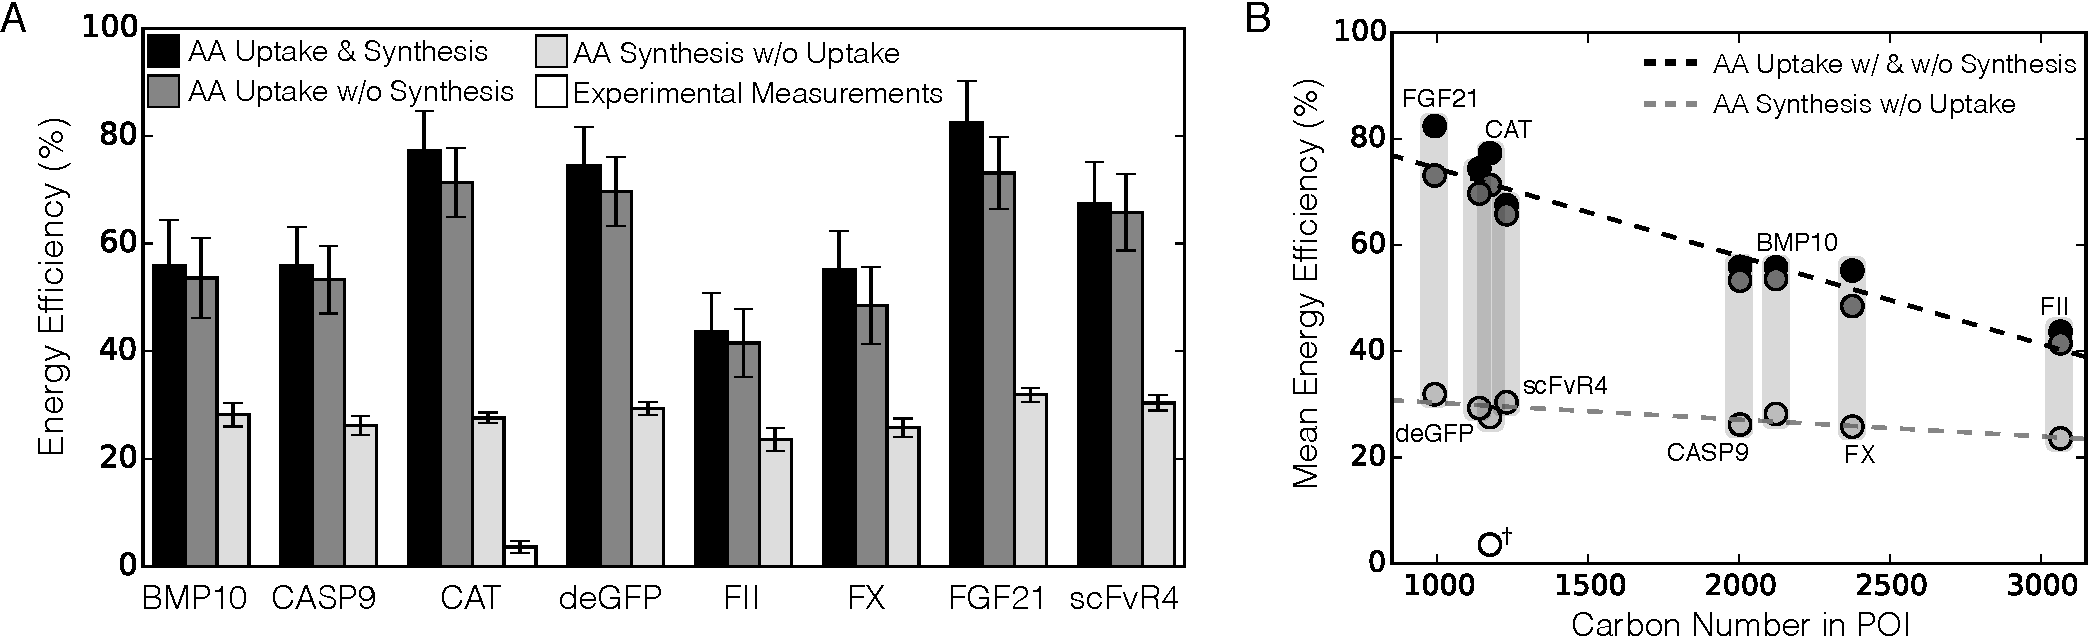
\includegraphics[width=1.00\textwidth]{./Figures/Energy.pdf}
% \caption{CFPS energy efficiency of eight proteins for four cases. Amino acid uptake and synthesis (black), AA uptake without synthesis (dark grey), AA synthesis without uptake (light grey), and constrained by experimental measurements, for CAT only (white). A. Energy efficiency (Error bars represent the 95\% CI of the ensemble). B. Mean energy efficiency versus the carbon number for each corresponding protein. Trendline of energy efficiency versus carbon number (black dotted line) for first two cases (y = -1.65$\cdot$10\textsuperscript{-2}x+90.95; R\textsuperscript{2} = 0.91) and trendline for AA synthesis without uptake (grey dotted line; y = -3.18$\cdot$10\textsuperscript{-3}x+33.48; R\textsuperscript{2} = 0.78). Dagger: constrained by experimental measurements and excluded from trendline.}
% \label{fig:Energy}
% \end{figure}

%To determine the carbon contribution from each substrate (glucose and amino acids) we examined the carbon flux going toward the production of deGFP for all three cases (Table \ref{tbl:yield_breakdown}).
%The cases supplemented with amino acids in the media showed the highest carbon yield.
%Finally, for the third case (without amino acids supplemented), the carbon yield was reduced to 51.1 $\pm$ 1.8\% for CAT, and the system used about twice the amount of glucose as in the first two cases.
%In this case, glucose was used to synthesize amino acids and provide the energy necessary to power transcription and translation; this trend was seen across all proteins.
% W, the system relied on a mixture of glucose and some amino acids for each protein with a carbon yield of 58.2 $\pm$ 2.3\% for CAT.
% Once amino acid synthesis reactions were blocked in the network (second case), the carbon yield dropped to 57.1 $\pm$ 2.2\% for CAT.

% If only the necessary amount of amino acids were used for the production of the protein of interest; thus, it may be hypothesized that all the glucose was used to power CFPS and did not contribute to the carbon yield.
% The carbon yield without the glucose contribution would be 100\%.

\subsubsection{Carbon yield}
The theoretical maximum carbon yield was inversely proportional to protein length and varied between 40\% to 64\% for the proteins sampled (Fig.~\ref{fig:Prof}E-F).
The relationship between the optimal carbon yield and carbon number was linear; $m_{Y}\times(C_{POI})+b_{Y}$ where $m_{Y} = -8.03\times10^{-3}$ carbon yield (\%)/carbon number with supplementation, and $m_{Y} = -6.98\times10^{-3}$ carbon yield (\%)/carbon number without supplementation.
The carbon yield (y-intercept) was $b_{Y} = 63.83$ (\%) with supplementation, and $b_{Y} = 58.86$ (\%) without supplementation.
The linear models of yield showed good ability to predict the optimal carbon yield for a range of carbon numbers ($R^{2} = 0.95$ with amino acid supplementation and $R^{2} = 0.90$ without supplementation), irrespective of the promoter used to control protein expression.
MBP also showed good agreement with the constraint based model, with a prediction error between 3\% and 4\% with and without amino acid supplementation.
The effective yield models were approximately parallel, with a drop in carbon yield of approximately 7\% without amino acids.
The difference between the cases was associated with a difference in glucose consumption.
In the absence of amino acids, glucose consumption increased, with the change in the carbon yield being largely accounted for by a change in CO\textsubscript{2} production.

The carbon yield for experimentally constrained CAT production was 6.2\% compared to the theoretical maximum of 58\% (Fig.~\ref{fig:Prof}F, dagger).
Given that the CAT productivity was similar between the simulated and measured systems, differences in the glucose consumption rate and byproduct accumulation were likely responsible for the difference between the optimal and experimental systems.
The translation rate has been identified as the rate-limiting step for cell-free protein synthesis \cite{2005_underwood_biotech,2014_li_PlosOne}, which was confirmed by the translation rate flux always hitting the upper bound in the simulation, regardless of protein.
Since CAT productivity could not be improved, the increased carbon consumption accumulated as byproducts: pyruvate, acetate, lactate, succinate and malate.
In addition, the accumulation of acetate and lactate suggested that oxidative phosphorylation activity was limited.
Thus, to improve carbon yield for CFPS, the translation rate should be improved for increased protein productivity, or energy efficiency should be improved to lower the glucose consumption rate.
%%%%%%%%%%%%%%%%%%%%
%However, it may also be hypothesized that only the amino acids supplied contribute to the carbon yield of the protein of interest, while glucose is used to energize CFPS.
%If this is the case, the carbon yield for the optimal and experimental systems resulted in approximately 100\%.
%%%%%%%%%%%%%%%%%%%%%

% \begin{figure}[t!]
% \centering
% 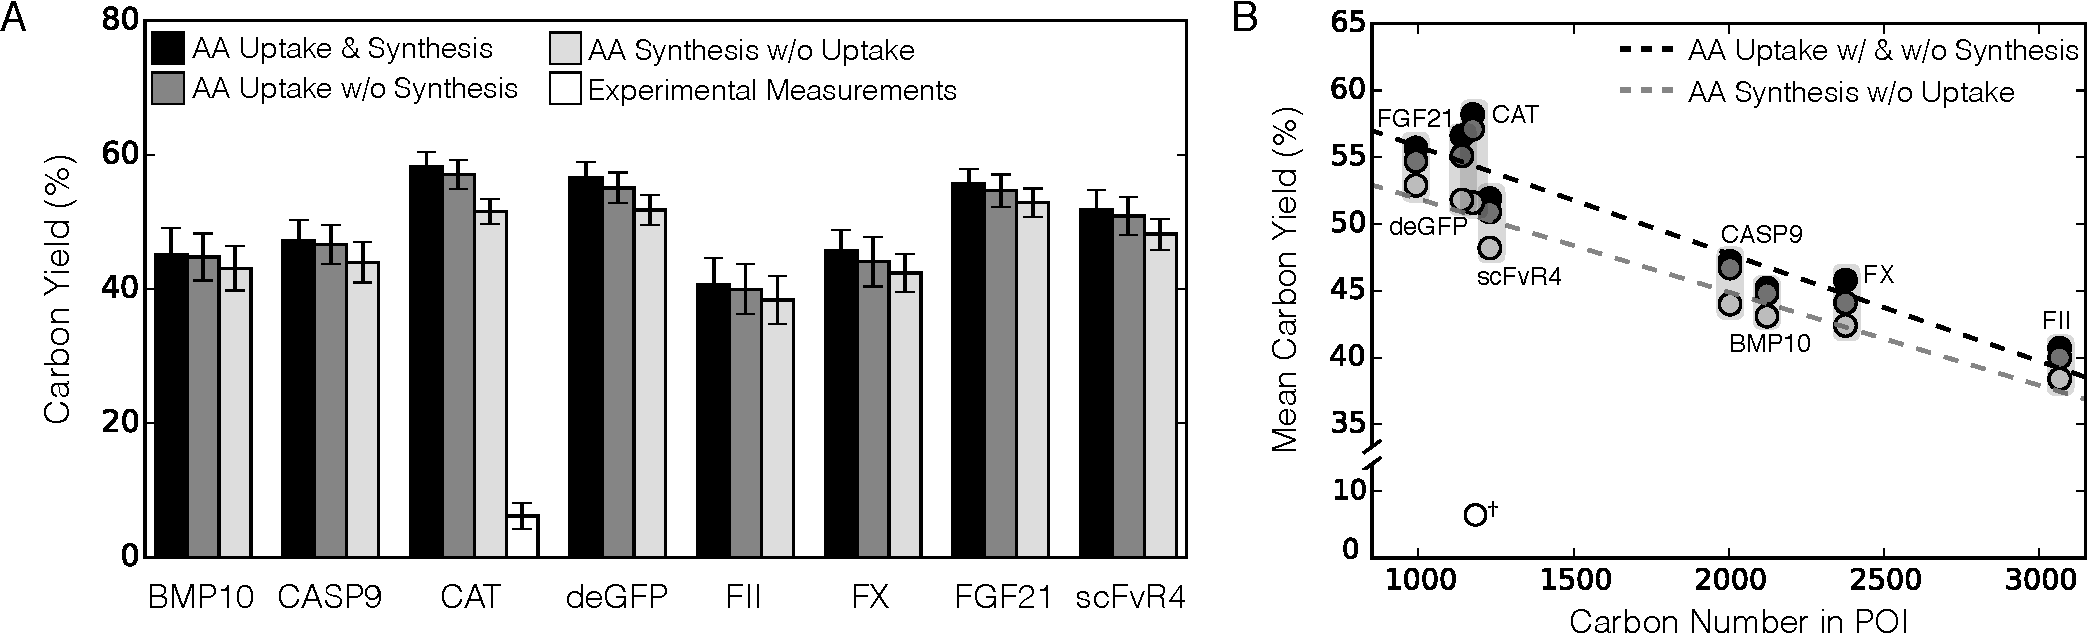
\includegraphics[width=1.00\textwidth]{./Figures/Yield.pdf}
% \caption{CFPS carbon yield of eight proteins for four cases. Amino acid uptake and synthesis (black), AA uptake without synthesis (dark grey), AA synthesis without uptake (light grey), and constrained by experimental measurements, for CAT only (white). A. Energy efficiency across the ensemble (error bars represent the 95\% CI). B. Mean energy efficiency versus the carbon number for each corresponding protein. Trendline of energy efficiency versus carbon number (black dotted line) for first two cases (y = -8.03$\cdot$10\textsuperscript{-3}x+63.83; R\textsuperscript{2} = 0.95) and trendline for AA synthesis without uptake (grey dotted line; y = -6.98$\cdot$10\textsuperscript{-3}x+58.86; R\textsuperscript{2} = 0.90). Dagger: constrained by experimental measurements and excluded from trendline.}
% \label{fig:Yield}
% \end{figure}
%Next we investigated the effect of the carbon number of each protein on the carbon yield (Fig.~\ref{fig:Yield}B).
%The proteins with the lowest carbon number had the highest yield and the higher carbon number proteins had a lower carbon yield within each case.
% A single trendline was formulated for the cases where amino acids were supplied in the media since they had similar performance, while another trendline was formulated for when amino acids were not available (Fig.~\ref{fig:Prof}F).

% Thus, we examined the parameters that had the most significant effect on cell-free productivity, energy efficiency, and carbon yield in order to optimize CFPS performance.

\subsection{Global sensitivity analysis}
To better understand the effect of substrate utilization and the transcription/translation parameters on CFPS performance, we performed global sensitivity analysis on the productivity, energy efficiency and carbon yield for the CAT protein (Fig.~\ref{fig:SI} and Fig. 1 in Supporting Information).
Surprisingly, RNAP and ribosome abundance had only a modest effect; the translation elongation rate had the largest effect on protein productivity.
On the other hand, oxygen and substrate consumption had the largest and second-largest influences on the energy efficiency and carbon yield, respectively.
The significance of transcription/translation parameters was robust to amino acid supplementation, with the translation rate being the most sensitive across all cases (Fig.~\ref{fig:SI}A).
This suggested that the translation elongation rate, and not transcriptional parameters, controlled productivity.
Underwood and coworkers showed that an increase in ribosome levels did not significantly increase protein yields or rates; however, adding elongation factors increased protein synthesis rates by 27\% \cite{2005_underwood_biotech}.
In addition, Li et al. increased the productivity by 5-fold of firefly luciferase in PURE CFPS by first improving the rate-limiting step, translation, followed by transcription by adjusting elongation factors, ribosome recycling factor, release factors, chaperones, BSA, and tRNAs \cite{2014_li_PlosOne}.
In examining substrate utilization, glucose consumption was not important for productivity in the presence of amino acid supplementation.
However, its importance increased significantly when amino acids were not available.
On the other hand, amino acid consumption was only sensitive when amino acids synthesis reactions were blocked, as it was the only source of amino acids for CAT synthesis.
The oxygen consumption rate was the most important factor controlling the energy efficiency of cell-free protein synthesis (Fig.~\ref{fig:SI}B).
In the model, we assumed that ATP could be produced by both substrate level and oxidative phosphorylation.
Jewett and coworkers reported that oxidative phosphorylation still operated in cell-free systems, and that the protein titer decreased from 1.5-fold to 4-fold when oxidative phosphorylation reactions were inhibited in pyruvate-powered CFPS \cite{Jewett:2008aa}.
However, it is unknown how active oxidative phosphorylation is in a glucose-powered cell-free system.
Moreover, the connection between oxidative phosphorylation activity and other performance metrics, such as carbon yield, is also unclear.

% The transcription/translation parameters had the same trend as for productivity, where the translation rate was the most sensitive compared to the other transcription/translation parameters and showed significance across all cases.
% In addition to the oxygen consumption, amino acid utilization was also sensitive.
% On the other hand, glucose consumption was only sensitive in the absence of amino acid supplementation,
% since glucose acted as the sole source of carbon and energy for protein synthesis.

To investigate the connection between carbon yield and oxidative phosphorylation further, we calculated the optimal CAT carbon yield as a function of the oxidative phosphorylation flux (Fig.~\ref{fig:oxphos_yield}).
Oxidative phosphorylation had a strong effect on the carbon yield, both with and without amino acid supplementation.
In the presence of amino acid supplementation, the carbon yield ranged from 20\% to approximately 60\%, depending on the oxidative phosphorylation flux.
However, without amino acid supplementation, the carbon yield dropped to approximately 10\%, and reached a maximum of 50\%.
In the absence of supplementation, a lower carbon yield was expected for the same oxidative phosphorylation flux, as glucose was utilized for both energy generation and amino acid biosynthesis.
In all cases, whenever the carbon yield was below its theoretical maximum, there was an accumulation of both acetate and lactate.
The experimental dataset exhibited a mixture of acetate and lactate accumulation during CAT synthesis, which suggested the CFPS reaction was not operating with optimal oxidative phosphorylation activity.
Oxidative phosphorylation is a membrane associated process, while CFPS has no cell membrane.
Jewett et al. hypothesized that membrane vesicles present in the CFPS reaction carry out oxidative phosphorylation \cite{Jewett:2008aa}.
In addition, they were able to enhance the production titer of CAT by 33\% when the reaction was augmented with 10mM phosphate.
However, it is unclear why the additional phosphate increased CAT yield.
Jewett et al. believe it either enhanced oxidative phosphorylation activity or inhibited phosphatase reactions.
The number, size, protein loading, and lifetime of these vesicles remains an open area of study.
Thus, we expect CFPS will have suboptimal oxidative phosphorylation capacity, and it remains an important area for optimization of CFPS performance.

% to both cases where amino acids were avaialbe.
% This drop in performance is due to the burden of synthesizing amino acids, which require NADPH.
% This leads to the relatively high flux in the first step of the pentose phosphate pathway to generate NADPH, thus, less NADH is available for oxidative phosphorylation.
% The performance metrics and sensitivity analysis suggest that efficient energy generation via oxygen uptake is essential to higher energy efficiency and carbon yields.
% %Thus, removing anaerobic enzymes during the cell-free extract preparation could potentially improve CFPS performance and protein yield.

\subsection{Optimal metabolic flux distribution}
Amino acid supplementation altered the optimal metabolic flux distribution predicted for CAT production (Fig.~\ref{fig:flux}).
To investigate the influence of amino acid supplementation, we compared the simulated metabolic flux distributions for CAT production with and without external amino acids.
In the presence of amino acid supplementation, and \textit{de~novo} amino acid synthesis, there was an incomplete TCA cycle, where a combination of glucose and amino acids powered protein expression (Fig.~\ref{fig:flux}A).
Glucose was consumed to produce acetyl-coenzyme A, and associated byproducts, while glutamate was converted to alpha-ketoglutarate which traveled to oxaloacetic acid and pyruvate for additional amino acid biosynthesis.
In the presence of amino acid supplementation, but without \textit{de~novo} amino acid biosynthesis, there was no TCA cycle flux.
In this case, ATP was produced by a combination of substrate level and oxidative phosphorylation, where ubiquinone was regenerated via \textit{nuo} activity, without relying on succinate dehydrogenase in the TCA cycle (Fig.~\ref{fig:flux}B).
These first two cases where amino acids were available had similar performance, and their respective metabolic flux distributions had a 99\% correlation for all proteins.
In the absence of amino acid supplementation (where all amino acids were synthesized \textit{de~novo} from glucose), the energy efficiency and carbon yield decreased; in this case, the TCA cycle was largely complete and there was diversion of metabolic flux into the Entner-Doudoroff pathway to produce NADPH (Fig.~\ref{fig:flux}C).
However, these simulations represent the theoretical optimum.
To more accurately describe the metabolic flux, we constrained the feasible solution space with experimental measurements and estimated the optimal CAT flux distribution.

The experimentally constrained optimal flux distribution had a 52\% correlation with the theoretically optimal flux distribution (Fig. \ref{fig:flux_exp}).
Metabolic fluxes were constrained by experimental measurements of glucose, amino and organic acid consumption and production rates for the first hour of the reaction (Supporting Information) and showed good agreement with the data with a coefficient of determination of R\textsuperscript{2}~=~0.92 (Fig.~\ref{fig:flux_exp}B).
The low similarity suggested several differences between the solutions which could be exploited to improve CFPS performance.
The largest discrepancy was in oxidative phosphorylation, where the experimental system relied heavily on \textit{cyd} rather than \textit{cyo}, which was less efficient for energy generation.
In addition, the experimental system had a high flux through \textit{zwf}, yielding an abundance of NADPH used for amino acid biosynthesis.
The remaining NADPH was interconverted to NADH via the \textit{pnt}1 reaction, which was consumed to convert pyruvate to lactate.
In contrast, the optimal solutions with amino acid supplementation had low activity in \textit{zwf} and \textit{pnt}1 reactions.
Folate, purine, and pyrimidine metabolism, along with amino acid biosynthesis, were inactive in the optimal system, but active in the experimental system.
In particular, the experimental system had high alanine and glutamine biosynthetic flux (both accumulated in the media), while there was no accumulation of amino acids in the optimal simulations.
Even though all amino acids were supplied in the reaction, glucose traveled through the major pathways and was utilized for amino acid biosynthesis.
Thus, it is unclear which substrate (glucose or amino acids) was used to power CFPS, and may likely be a combination of both.
Lastly, the optimal solution produced (or consumed) only the required amount of amino acids;
meanwhile,  alanine, glutamine, pyruvate, lactate, acetate, malate, and succinate all accumulated in the experimental system.
This accumulation contributed to the difference in flux distribution.

% the experimental system there was an accumulation of  which contributed to some of the differences in the flux distributions. % and may have contributed to the inefficiency of carbon utilization.

\subsubsection{Potential alternative metabolic optima}
Optimal flux distributions predicted using constraint based approaches may not always be unique.
Alternative optimal solutions have the same objective value, e.g., productivity, but different metabolic flux distributions.
Techniques such as flux variability analysis (FVA) \cite{Mahadevan2003264,Schuetz:2007aa} or mixed-integer approaches \cite{LEE2000711} can estimate alternative optima.
In this study, we used group knockout analysis to estimate potential alternative optimal solutions for CAT production constrained by experimental measurements (Fig.~\ref{fig:norm}).
Groups of reactions were removed from the metabolic network, and the translation rate was maximized.
The difference between the nominal and altered system was then calculated.
Knockout analysis identified pathways required for CAT production; for example, deletion of the glycolysis/gluconoeogenesis or oxidative phosphorylation pathways resulted in no CAT production.
Likewise, there were pathway knockouts that had no effect on productivity or the metabolic flux distribution, such as removal of isoleucine, leucine, histidine and valine biosynthesis.
Globally, the constraint based simulation reached the same optimal CAT productivity for 40\% of the pairwise knockouts, while 92\% of these solutions had different flux distributions compared with the wild-type.
For example, one of the features of the predicted optimal metabolic flux distribution was a high flux through the Entner-Douodoroff (ED) pathway.
Removal of the ED pathway had no effect on the CAT productivity compared to the absence of knockouts (Fig.~\ref{fig:norm}A).
Pairwise knockouts of the ED pathway and other subgroups (i.e. pentose phosphate pathway, cofactors, folate metabolism, etc.) also resulted in the same optimal CAT productivity.
However, there was a difference in the flux distribution with these knockouts (Fig.~\ref{fig:norm}B); thus, alternative optimal metabolic flux distributions exist for CAT production, despite experimental constraints.
In addition, knockouts of amino acid biosynthesis reactions had no effect on the productivity with the exception of alanine, aspartate, asparagine, glutamate and glutamine biosynthesis reactions, since amino acids were available in the media.
Ultimately, to determine the metabolic flux distribution occurring in CFPS, we need to add additional constraints to the flux estimation calculation.
For example, thermodynamic feasibility constraints may result in a better depiction of the flux distribution \cite{Henry:2007,Hamilton:2013}, and $^{13}$C labeling in CFPS could provide significant insight.
However, while $^{13}$C labeling techniques are well established for \emph{in~vivo} processes \cite{Zamboni:2009}, application of these techniques to CFPS remains an active area of research.

% Despite the constraints by experimental measurements, it is difficult to calculate the physiological flux distribution of metabolism (Fig.~\ref{fig:norm})
% For example, there is a high flux through the Entner-Douodoroff pathway, but this may be an artifact of the optimal solution.
% Flux balance analysis has been shown to have multiple alternative optimal solutions with flux variablitiy analysis and mixed-integer linear programming resulting in a poor depiction of the physiological flux distribution \cite{LEE2000711, Mahadevan2003264, Schuetz119}.

\subsection{Summary and conclusions}
In this study, we developed a sequence specific constraint based modeling approach to predict the performance of cell-free protein synthesis reactions for a range of proteins.
First principle predictions of the cell-free production of deGFP and CAT were in agreement with experimental measurements, for two different promoters.
Here we considered only the P70a and T7 promoters, but we are currently expanding our library of possible promoters.
A library of computational promoters, in combination with the cell-free constraints based approach,
could enable the \emph{de~novo} design of circuits for optimal functionality and performance.
We also developed effective correlation models for the productivity, energy efficiency and carbon yield as a function of protein size.
Simulations of maltose binding protein expression showed good agreement with these correlation models, suggesting the effective correlations could be used to quickly prototype CFPS reactions.
Further, global sensitivity analysis identified the key metabolic processes that controlled CFPS performance;
oxidative phosphorylation was vital to energy efficiency and carbon yield, while the translation rate was the most important for productivity.
However, ATP was predicted to be produced by both substrate level and oxidative phosphorylation, as both lactate and acetate accumulated in the experimental system.
While the results of this first study were promising, there are several issues to consider in future work.
First, a more detailed description of transcription and translation reactions that has been utilized in other genome scale ME models e.g., O’Brien et al \cite{Brien693} could be adapted
to a cell-free system. This would allow us to consider important facets of protein production, such as the role of chaperones in protein folding.
We would also like to include post-translation modifications such as glycosylation that are important for the production of therapeutic proteins.
In conclusion, sequence specific constraint based modeling of cell-free protein production offers a novel means to \emph{a~priori}
estimate the optimal performance of cell-free synthetic circuits.

% required for proper protein folding and functionality.
%

\clearpage

\section*{Materials and Methods}

\subsection*{Glucose/NMP cell-free protein synthesis.}
The glucose/NMP cell-free protein synthesis reaction was
performed using the S30 extract in 1.5-mL Eppendorf tubes (working volume of 15 $\mu$L) and incubated in a humidified incubator.
The S30 extract was prepared from \textit{E.~coli} strain KC6 (A19 $\Delta$tonA $\Delta$tnaA $\Delta$speA $\Delta$endA $\Delta$sdaA $\Delta$sdaB $\Delta$gshA met+).
This K12-derivative has several gene deletions to stabilize amino acid concentrations during the cell-free reaction.
The KC6 strain was grown to approximately 3.0 OD595 in a 10-L fermenter (B. Braun, Allentown PA) on defined media with glucose as the carbon source and with the addition of 13 amino acids (alanine, arginine, cysteine, serine, aspartate, glutamate, and glutamine were excluded) \cite{Zawada:2003}. Crude S30 extract was prepared as described previously \cite{Jewett:2002}.
Plasmid pK7CAT was used as the DNA template for chloramphenical acetyl transferase (CAT) expression by placing the \emph{cat} gene
between the T7 promoter and the T7 terminator \cite{Kigawa1995}.
The plasmid was isolated and purified using a Plasmid Maxi Kit (Qiagen, Valencia CA).
Cell-free CAT synthesis was performed at 37 $^{\circ}$C.

The protein synthesis reaction was conducted using the PANOxSP protocol with slight modifications from that described previously \cite{BIT:BIT20026}.
Unless otherwise noted, all reagents were purchased from Sigma (St. Louis, MO).
The initial mixture included 1.2 mM ATP; 0.85 mM each of GTP, UTP, and CTP; 30 mM phosphoenolpyruvate (Roche, Indianapolis IN); 130 mM potassium glutamate; 10 mM ammonium glutamate; 16 mM magnesium glutamate; 50 mM HEPES-KOH buffer (pH 7.5); 1.5 mM spermidine; 1.0 mM putrescine; 34 $\mu$g/mL folinic acid; 170.6 $\mu$g/mL \textit{E.~coli} tRNA mixture (Roche, Indianapolis IN); 13.3 $\mu$g/mL pK7CAT plasmid; 100 $\mu$g/mL T7 RNA polymerase; 20 unlabeled amino acids at 2-3 mM each; 5 $\mu$M l-[U-\textsuperscript{14}C]-leucine (Amersham Pharmacia, Uppsala Sweden); 0.33 mM nicotinamide adenine dinucleotide (NAD); 0.26 mM coenzyme A (CoA); 2.7 mM sodium oxalate; and 0.24 volumes of \textit{E.~coli} S30 extract.
This reaction was modified for the energy source used such that glucose reactions have 30-40 mM glucose in place of PEP.
Sodium oxalate was not added since it has a detrimental effect on protein synthesis and ATP concentrations when using glucose or other early glycolytic intermediate energy sources \cite{BIT:BIT1121}. The HEPES buffer (pKa $\sim$ 7.5) was replaced with Bis-Tris (pKa $\sim$ 6.5). In addition, the magnesium glutamate concentration was reduced to 8 mM for the glucose reaction since a lower magnesium optimum was found when using a nonphosphorylated energy source \cite{BIT:BIT20026}. Finally, 10 mM phosphate was added in the form of potassium phosphate dibasic adjusted to pH 7.2 with acetic acid.

\subsection*{Protein product and metabolite measurements.}
Cell-free reaction samples were quenched at specific timepoints with equal volumes of ice-cold 150 mM sulfuric acid to precipitate proteins.
Protein synthesis of CAT was determined from the total amount of \textsuperscript{14}C-leucine-labeled product by trichloroacetic acid precipitation followed by scintillation counting as described previously \cite{2005_calhoun_BiotechnologyProgress}.
Samples were centrifuged for 10 min at 12,000g and 4$^{\circ}$C.
The supernatant was collected for high performance liquid chromatography (HPLC) analysis.
HPLC analysis (Agilent 1100 HPLC, Palo Alto CA) was used to separate nucleotides and organic acids, including glucose. Compounds were identified and quantified by comparison to known standards for retention time and UV absorbance (260 nm for nucleotides and 210 nm for organic acids) as described previously \cite{2005_calhoun_BiotechnologyProgress}.
The standard compounds quantified with a refractive index detector included inorganic phosphate, glucose, and acetate.
Pyruvate, malate, succinate, and lactate were quantified with the UV detector.
The stability of the amino acids in the cell extract was determined using a Dionex Amino Acid Analysis (AAA) HPLC System (Sunnyvale, CA) that separates amino acids by gradient anion exchange (AminoPac PA10 column).
Compounds were identified with pulsed amperometric electrochemical detection and by comparison to known standards.

\subsection*{Formulation and solution of the model equations.}
The sequence specific flux balance analysis problem was formulated as a linear program:
\begin{equation}
 \begin{multlined}
	\qquad \qquad \qquad \max_{\boldsymbol{w}}{} \! \left( w_{X} = \mathbf{\boldsymbol{\theta}}^T \boldsymbol{w} \right) \\
	\mathrm{Subject \; to:}
	 \; \; \mathbf{S}\mathbf{w}=\mathbf{0} \\
\mathcal{L}_{i} \leq w_i \leq \mathcal{U}_{i}  \qquad i=1,2,\hdots,\mathcal{R}
 \end{multlined}
\end{equation}
where $\mathbf{S}$ denotes the stoichiometric matrix, $\mathbf{w}$ denotes the unknown flux vector, $\boldsymbol{\theta}$ denotes the objective cost vector
and $\mathcal{L}_{i}$ and $\mathcal{U}_{i}$ denote the lower and upper bounds on flux $w_{i}$, respectively.
The transcription (T) and translation (X) stoichiometry was modeled based upon the template reactions of Allen and Palsson \cite{Allen:2003aa} (Table \ref{tbl:template-reactions}).
The objective of the sequence specific flux balance calculation was to maximize the rate of protein translation, $w_{X}$.
The total glucose uptake rate was bounded by [0,40 mM/h] according to experimental data, while the amino acid uptake rates were bounded by [0,30 mM/h], but did not reach the maximum flux.
Gene and protein sequences were taken from literature and are available in the Supporting Information.
The sequence specific flux balance linear program was solved using the GNU Linear Programming Kit (GLPK) v4.55 \cite{GLPK}.
For all cases, amino acid degradation reactions were blocked as these enzymes were likely inactivated during the cell-free extract preparation \cite{2005_calhoun_BiotechnologyProgress, Garamella:2016aa}.
In the absence of \textit{de~novo} amino acid synthesis, all amino acid synthesis reactions were set to 0 mM/hr.
In the experimentally constrained simulations, \textit{E. coli} was grown in the presence of 13 amino acids (alanine, arginine, cysteine, serine, aspartate, glutamate, and glutamine were excluded) \cite{Zawada:2003}, thus the synthesis reactions responsible for those 13 amino acids were set to 0 mM/hr.


% We estimated the theoretical maximum performance of the cell-free protein synthesis system using sequence specific flux balance analysis (ssFBA) \cite{Allen:2003aa}.
% The sequence specific flux balance analysis problem was formulated as a linear program:
% \begin{equation}
%  \begin{multlined}
% 	\qquad \qquad \qquad \max_{\boldsymbol{w}}{} \! \left( w_{TL} = \mathbf{\boldsymbol{\theta}}^T \boldsymbol{w} \right) \\
% 	\mathrm{Subject \; to:}
% 	 \; \; \mathbf{S}\mathbf{w}=\mathbf{0} \\
% \alpha_i \leq w_i \leq \beta_i  \qquad i=1,2,\hdots,\mathcal{R}
%  \end{multlined}
% \end{equation}
% where $\mathbf{S}$ denotes the stoichiometric matrix, $\mathbf{w}$ denotes the unknown flux vector, $\boldsymbol{\theta}$ denotes the objective selection vector
% and $\alpha_i$ and $\beta_i$ denote the lower and upper bounds on flux $w_{i}$, respectively.
% The stoichiometry of the kinetic model was used for the ssFBA calculations, with the execpetion of the transcription and translation rates.
% The transcription (TX) and translation (TL) stoichiometry was modeled using the template reactions taken from Allen and Palsson \cite{Allen:2003aa}:
% \begin{eqnarray*}
% \mathrm{{G}_{\mathcal{P}}}+\mathrm{{R}_{1}} &\longrightarrow& \mathrm{G_{\mathcal{P}}^{*}} \\
% \mathrm{G_{\mathcal{P}}^{*}}+\sum_{\mathrm{k\in\left\{A,C,G,U\right\}}}\eta_{k}\cdot \mathrm{\left\{k\right\}TP} &\overset{\rm TX}{\longrightarrow}& \mathrm{mRNA}+\mathrm{G_{\mathcal{P}}}+\mathrm{R_{T}}+ \mathrm{\sum_{k\in\left\{A,C,G,U\right\}}2\eta_{k}\cdot Pi}\\
% \mathrm{mRNA} &\longrightarrow& \mathrm{\sum_{k\in\left\{A,C,G,U\right\}}\eta_{k}\cdot \left\{k\right\}MP} \\
% \mathrm{mRNA}+\mathrm{R_{X}} &\longrightarrow& \mathrm{R_{X}^{*}} \\
% \mathrm{\alpha_{j}\cdot AA_{j}+\alpha_{j}\cdot tRNA+\alpha_{j}\cdot ATP} &\longrightarrow& \mathrm{\alpha_{j}\cdot AA_{j}-tRNA_{j}+}\\
% && \mathrm{\qquad \alpha_{j}\cdot AMP+2\alpha_{j}\cdot Pi} \qquad{j=1,2,\hdots,20}\\
% \mathrm{R_{X}^{*}+\sum_{j\in\left\{AA\right\}}\alpha_{j}\cdot \Big(AA_{j}-tRNA_{j}+2\cdot GTP\Big)} &\stackrel{\rm TL}{\longrightarrow}& \mathcal{P}+\mathrm{R_{X}+mRNA}+\\
% && \mathrm{\quad +\sum_{j\in\left\{AA\right\}}\alpha_{j}\cdot\Big(tRNA+2\cdot GDP+2\cdot Pi\Big)}
% \end{eqnarray*}
% where $G_{\mathcal{P}}$ denotes the gene encoding protein product $\mathcal{P}$,
% $\rm R_{T}$ denotes the concentration of RNA polymerase,
% $G_{\mathcal{P}}^{*}$ denotes the gene bounded by the RNA polymerase,
% $\eta_{i}$ and $ \alpha_{j}$ denote the stoichiometric coefficients for nucleotide and amino acid, respectively,
% $\rm Pi$ denotes inorganic phosphate,
% $\rm R_{X}$ denotes the ribosome concentration,
% $\rm R_{X}^{*}$ denotes bounded ribosome,
% and $AA_{j}$ denotes the $j^{th}$ amino acid.

The bounds on the transcription rate ($\mathcal{L}_{T}=w_{T}=\mathcal{U}_{T}$) were modeled as:
\begin{equation}
	w_{T} = V_{T}^{max}\left(\frac{G_{\mathcal{P}}}{K_{T}+G_{\mathcal{P}}}\right)
\end{equation}
where $G_{\mathcal{P}}$ denotes the gene concentration of the protein of interest, and $K_{T}$ denotes a transcription saturation coefficient.
The maximum transcription rate $V_{T}^{max}$ was formulated as:
\begin{equation}
	V_{T}^{max} \equiv \left[R_{T}\left(\frac{\dot{v}_{T}}{l_{G}}\right)u\left(\kappa\right)\right]
\end{equation}
The term $R_{T}$ denotes the RNA polymerase concentration (nM),
$\dot{v}_{T}$ denotes the RNA polymerase elongation rate (nt/h),
$l_{G}$ denotes the gene length in nucleotides (nt).
The term $u\left(\kappa\right)$ (dimensionless, $0\leq u\left(\kappa\right)\leq 1$)
is an effective model of promoter activity, where $\kappa$ denotes promoter specific parameters.
The general form for the promoter models was taken from Moon $\emph{et~al.}$ \cite{Moon:2012ab}.
In this study, we considered two promoters: T7 and P70a.
The promoter function for the T7 promoter, $u_{T7}$, was given by:
\begin{equation}
	u_{T7} = \frac{K_{T7}}{1 + K_{T7}}
\end{equation}
where $K_{T7}$ denotes a T7 RNA polymerase binding constant.
The P70a promoter function $u_{P70a}$ (which was used for all other proteins) was formulated as:
\begin{equation}
	u_{P70a} = \frac{K_{1}+K_{2}f_{\sigma_{70}}}{1 + K_{1}+K_{2}f_{\sigma_{70}}}
\end{equation}
where $K_{1}$ denotes the weight of RNA polymerase binding alone,
$K_{2}$ denotes the weight of RNAP-$\sigma_{70}$ bound to the promoter,
and $f_{p70}$ denotes the fraction of the $\sigma_{70}$ transcription factor bound to RNAP, modeled as a Hill function:
\begin{equation}
	f_{\sigma_{70}} = \frac{\sigma_{70}^{n}}{K_{D}^{n} + \sigma_{70}^{n}}
\end{equation}
where $\sigma_{70}$ denotes the sigma-factor 70 concentration, $K_{D}$ denotes the dissociation constant, and $n$ denotes a cooperativity coefficient.
The values for all promoter parameters are given in Table ~\ref{tbl:parameters}.

The translation rate ($w_{X}$) was bounded by:
 \begin{equation}
	0\leq w_{X} \leq V_{X}^{max}\left(\frac{mRNA^{*}}{K_{X}+mRNA^{*}}\right)
\end{equation}
where $\rm mRNA^{*}$ denotes the steady state mRNA abundance and $K_{X}$ denotes a translation saturation constant.
The maximum translation rate $V_{X}^{max}$ was formulated as:
\begin{equation}
	V_{X}^{max} \equiv \left[K_{P} R_{X}\left(\frac{\dot{v}_{X}}{l_{P}}\right)\right]
\end{equation}
The term $K_{P}$ denotes the polysome amplification constant,
$\dot{v}_{X}$ denotes the ribosome elongation rate (amino acids per hour),
$l_{P}$ denotes the number of amino acids in the protein of interest.
The steady state mRNA abundance $\rm mRNA^{*}$ was estimated as:
\begin{equation}
	 mRNA^{*}\simeq\frac{w_{T}}{\lambda}
\end{equation}
where $\lambda$ denotes the rate constant controlling the mRNA degradation rate (hr$^{-1}$).
All translation parameters are given in Table \ref{tbl:parameters}.

\subsection*{Calculation of energy efficiency.}
Energy efficiency ($\mathcal{E}$) was calculated as the ratio of protein production to glucose consumption, written in terms of equivalent ATP molecules:
\begin{equation}\label{eqn:energy-efficiency-definition}
	\mathcal{E}\equiv\frac{w_{X}\left(2\cdot\rm {ATP}_{X}+\rm {GTP}_{X}\right)+w_{T}\left(2\times\left(\rm {ATP}_{T}+\rm {CTP}_{T}+\rm {GTP}_{T}+\rm {UTP}_{T}\right) \right)}{\rm{q}_{GLC}\cdot\rm{ATP}_{GLC}}
\end{equation}
where $\rm {ATP}_{T}$, $\rm {CTP}_{T}$, $\rm {GTP}_{T}$, $\rm {UTP}_{T}$ denote the stoichiometric coefficients of each energy species for the transcription of the protein of interest, $\rm {ATP}_{X}$, $\rm {GTP}_{X}$ denote the stoichiometric coefficients of ATP and GTP for the translation of the protein of interest, $\rm{q}_{GLC}=w_{GLC}$ denotes the glucose uptake rate,
and $\rm{ATP}_{GLC}$ denotes the equivalent ATP number produced per glucose.
The energy species stoichiometric coefficients are available in the Supporting Information.

\subsection*{Calculation of the carbon yield.}
The carbon yield ($Y_{C}^{POI}$) was calculated as the ratio of carbon produced as the protein of interest divided by the carbon consumed as reactants (glucose and amino acids):
\begin{equation}\label{eqn:yield-definition}
	Y_{C}^{POI}\equiv\frac{\texttt{q}_{POI}\cdot C_{POI}}{\displaystyle\sum_{i=1}^{\mathcal{R}} \texttt{q}_{m_{i}}\cdot C_{m_i}}
\end{equation}
where $\texttt{q}_{POI}$ denotes the flux of the protein of interest produced, $C_{POI}$ denotes carbon number of the protein of interest, $\mathcal{R}$ denotes the number of reactants,
$\texttt{q}_{m_{i}}$ denotes the uptake flux of the $i^{th}$ reactant, and $C_{m_i}$ denotes the carbon number of the $i^{th}$ reactant.


\subsection*{Quantification of uncertainty.}
Experimental factors taken from literature, for example macromolecular concentrations or elongation rates, are uncertain.
To quantify the influence of this uncertainty on model performance, we randomly sampled the expected physiological ranges for these parameters as determined from literature.
An ensemble of flux distributions was calculated for the three different cases we considered:
control (with amino acid synthesis and uptake), amino acid uptake without synthesis, and amino acid synthesis without uptake.
The flux ensemble was calculated by randomly sampling the maximum glucose consumption rate within a range of 0 to 30 mM/h, (determined from experimental data)
and randomly sampling RNA polymerase levels, ribosome levels, and elongation rates in a physiological range determined from literature.
RNA polymerase levels were sampled between 60 and 80 nM, ribosome levels between 12 and 18 \textmu M, the RNA polymerase elongation rate between 20 and 30 nt/sec, and the ribosome elongation rate between 1.5 and 3 aa/s \cite{2005_underwood_biotech, Garamella:2016aa}.

\subsection*{Global sensitivity analysis.}
We conducted a global sensitivity analysis using the variance-based method of Sobol to estimate which parameters controlled the performance of the cell-free protein synthesis reaction \citep{SOBOL_METHOD}.
We computed the total sensitivity index of each parameter relative to three performance objectives: productivity of the protein of interest, energy efficiency and carbon yield.
We established the sampling bounds for each parameter from literature.
We used the sampling method of Saltelli \textit{et al.} \citep{Saltelli:2010} to compute a family of $N\left(2d+2\right)$ parameter sets which obeyed our parameter ranges,
where $N$ was a parameter proportional to the desired number of model evaluations and $d$ was the number of parameters in the model. In our case, $N$ = 1000 and $d$ = 7, so the total sensitivity indices were computed from 16,000 model evaluations. The variance-based sensitivity analysis was conducted using the SALib module encoded in the Python programming language \citep{SALIB}.

\subsection*{Potential alternative optimal metabolic flux solutions.}
We identified potential alternative optimal flux distributions by performing single and pairwise reaction group knockout simulations.
Reaction group knockouts were simulated by setting the flux bounds for all the reactions involved in a group to zero and then maximizing the translation rate.
We grouped reactions in the cell-free network into 19 subgroups (available in Supporting Information).
We computed the difference ($l^{2}$-norm) for CAT productivity in the presence and absence of pairwise reaction knockouts.
Simultaneously, we computed the difference in the flux distribution ($l^{2}$-norm) for each pairwise reaction knockout compared to the flux distribution with no knockouts.
Those solutions with the same or similar productivity but large changes in the metabolic flux distribution represent alternative optimal solutions.

%%%%%%%%%%%%%%%%%%%%%%%%%%%%%%%%%%%%%%%%%%%%%%%%%%%%%%%%%%%%%%%%%%%%%
%% The "Acknowledgement" section can be given in all manuscript
%% classes.  This should be given within the "acknowledgement"
%% environment, which will make the correct section or running title.
%%%%%%%%%%%%%%%%%%%%%%%%%%%%%%%%%%%%%%%%%%%%%%%%%%%%%%%%%%%%%%%%%%%%%
\begin{acknowledgement}

This study was supported by an award from the US Army and Systems Biology of Trauma Induced Coagulopathy (W911NF-10-1-0376) to J.V. for the support of M.V.
The work was also supported by the Center on the Physics of Cancer Metabolism through Award Number 1U54CA210184-01 from the National Cancer Institute.
The content is solely the responsibility of the authors and does not necessarily represent the official views of the National Cancer Institute or the National Institutes of Health.

\end{acknowledgement}

%%%%%%%%%%%%%%%%%%%%%%%%%%%%%%%%%%%%%%%%%%%%%%%%%%%%%%%%%%%%%%%%%%%%%
%% The same is true for Supporting Information, which should use the
%% suppinfo environment.
%%%%%%%%%%%%%%%%%%%%%%%%%%%%%%%%%%%%%%%%%%%%%%%%%%%%%%%%%%%%%%%%%%%%%
\begin{suppinfo}
The following files are available free of charge.
\begin{itemize}
  \item Protein Sequences: DNA and protein sequences of each protein of interest.
  \item Supporting Information: Performance trendlines as a function of carbon number, transcription/translation stoichiometric coefficients of energy species, and experimental measurements of CAT production.
  \item Carbon Yield Sensitivity Analysis: Global sensitivity analysis on deGFP carbon yield.
  \item Metabolites and reactions of the cell-free stoichiometric network.
\end{itemize}
\end{suppinfo}

\clearpage

%%%%%%%%%%%%%%%%%%%%%%%%%%%%%%%%%%%%%%%%%%%%%%%%%%%%%%%%%%%%%%%%%%%%%
%% The appropriate \bibliography command should be placed here.
%% Notice that the class file automatically sets \bibliographystyle
%% and also names the section correctly.
%%%%%%%%%%%%%%%%%%%%%%%%%%%%%%%%%%%%%%%%%%%%%%%%%%%%%%%%%%%%%%%%%%%%%

\begin{table}
\centering
    \caption{Transcription and translation template reactions for protein production. The symbol $G_{\mathcal{P}}$ denotes the gene encoding protein product $\mathcal{P}$,
    $R_{T}$ denotes the concentration of RNA polymerase,
    $G_{\mathcal{P}}^{*}$ denotes the gene bounded by the RNA polymerase (open complex),
    $\eta_{i}$ and $ \alpha_{j}$ denote the stoichiometric coefficients for nucleotide and amino acid, respectively,
    $Pi$ denotes inorganic phosphate,
    $R_{X}$ denotes the ribosome concentration,
    $R_{X}^{*}$ denotes bound ribosome,
    and $AA_{j}$ denotes $j^{th}$ amino acid.}
    \renewcommand{\arraystretch}{1.2}
    \resizebox{\textwidth}{!}{\begin{tabular}{llcl} \toprule
        \textbf{Description} & \multicolumn{3}{l}{\textbf{Template reaction}} \\ \toprule
        Transcription initiation & $G_\mathcal{P}+R_{T}$ & $\longrightarrow$& $G_{\mathcal{P}}^{*}$ \\
        Transcription ($w_{T}$) & $G_{\mathcal{P}}^{*}+\quad\displaystyle\sum_{\mathclap{k\in\left\{A,C,G,U\right\}}}\eta_{k}\cdot \left(\left\{k\right\}TP + H_{2}O\right)$ & $\longrightarrow$& $mRNA+G_{\mathcal{P}}+R_{T}+\displaystyle\sum_{\mathclap{k\in\left\{A,C,G,U\right\}}} \eta_{k} \cdot PPi$ \\
        mRNA degradation &  $mRNA$ &$\longrightarrow$& \quad $\displaystyle\sum_{\mathclap{k\in\left\{A,C,G,U\right\}}}\eta_{k}\cdot \left\{k\right\}MP$ \\
	Translation initiation & $mRNA+R_{X}$ &$\longrightarrow$& $R_{X}^{*}$ \\
        tRNA charging & $\alpha_{j}\cdot \Big(AA_{j}+tRNA+ATP+H_{2}O\Big)$ &$\longrightarrow$& $\alpha_{j}\cdot \Big(AA_{j}\text{-}tRNA_{j} +AMP+PPi\Big)$ \\
 	&&& $\qquad \qquad \qquad \qquad \quad  {j=1,2,\hdots,20}$\\
        Translation ($w_{X}$) &  $R_{X}^{*}+\displaystyle\sum_{\mathclap{j\in\left\{AA\right\}}}\alpha_{j}\cdot \Big(AA_{j}\text{-} tRNA_{j}+2GTP+2H_{2}O\Big)$ &$\longrightarrow$& $\mathcal{P}+R_{X}+mRNA$\\
&&& $\quad +\displaystyle\sum_{\mathclap{j\in\left\{AA\right\}}}\alpha_{j}\cdot\Big(tRNA+2GDP+2Pi\Big)$ \\ \bottomrule
    \end{tabular}}
\label{tbl:template-reactions}
\end{table}

\clearpage

\begin{table}
\centering
    \caption{Parameters for sequence specific flux balance analysis}
    \renewcommand{\arraystretch}{1}
    \begin{tabular}{lcccc} \toprule
        \textbf{Description} & \textbf{Parameter} & \textbf{Value} & \textbf{Units} & \textbf{Reference} \\ \toprule
        RNA polymerase concentration & $R_{T}$ & 75 & nM & \cite{Garamella:2016aa} \\
        Ribosome concentration & $R_{X}$ & 1.6 & $\mu$M & \cite{Garamella:2016aa, 2005_underwood_biotech} \\

        & & & & \\
        Transcription elongation rate & $\dot{v}_{T}$ & 25 & nt/sec & \cite{Garamella:2016aa} \\
        Translation elongation rate & $\dot{v}_{X}$ & 2 & aa/sec & \cite{Garamella:2016aa, 2005_underwood_biotech} \\
        Transcription saturation coefficient & $K_{T}$ & 3.5 & nM & estimated \\
        Translation saturation coefficient & $K_{X}$ & 45.0 & $\mu$M & estimated \\
        Polysome amplification constant & $K_{P}$ & 10 & constant & estimated \\
        mRNA degradation rate & $\lambda$ & 5.2 & hr\textsuperscript{-1} & \cite{Garamella:2016aa} \\

        & & & & \\
        T7 promoter & $K_{T7}$ & 10 & constant & estimated \\
        Weight RNA polymerase binding alone P70a & $K_{1}$ & 0.014 & constant & estimated \\
        Weight bound RNAP-$\sigma_{70}$ P70a & $K_{2}$ & 10 & constant & estimated \\
        $\sigma_{70}$ concentration & $\sigma_{70}$ & 35 & nM & \cite{Garamella:2016aa} \\
        $\sigma_{70}$ dissociation constant & $K_{D}$ & 130 & nM & \cite{Mauri:2014aa} \\
	      $\sigma_{70}$ hill coefficient & n & 1 & constant & \cite{Mauri:2014aa} \\
        Gene concentration & $G_{\mathcal{P}}$ & 5 & nM &  \cite{Garamella:2016aa} \\ \bottomrule

        % & & & & \\
	      %
        % Gene length of CAT & $l_{G}$ & 683 & nt & \cite{Kigawa1995} \\
        % Gene length of deGFP & $l_{G}$ & 660 & nt & \cite{Garamella:2016aa} \\
        % Protein length of CAT & $l_{P}$ & 229 & aa & \cite{Kigawa1995} \\
        % Protein length of deGFP & $l_{P}$ & 219 & aa & \cite{Garamella:2016aa} \\
    \end{tabular}
\label{tbl:parameters}
\end{table}

\clearpage

\begin{figure}[t!]
\centering
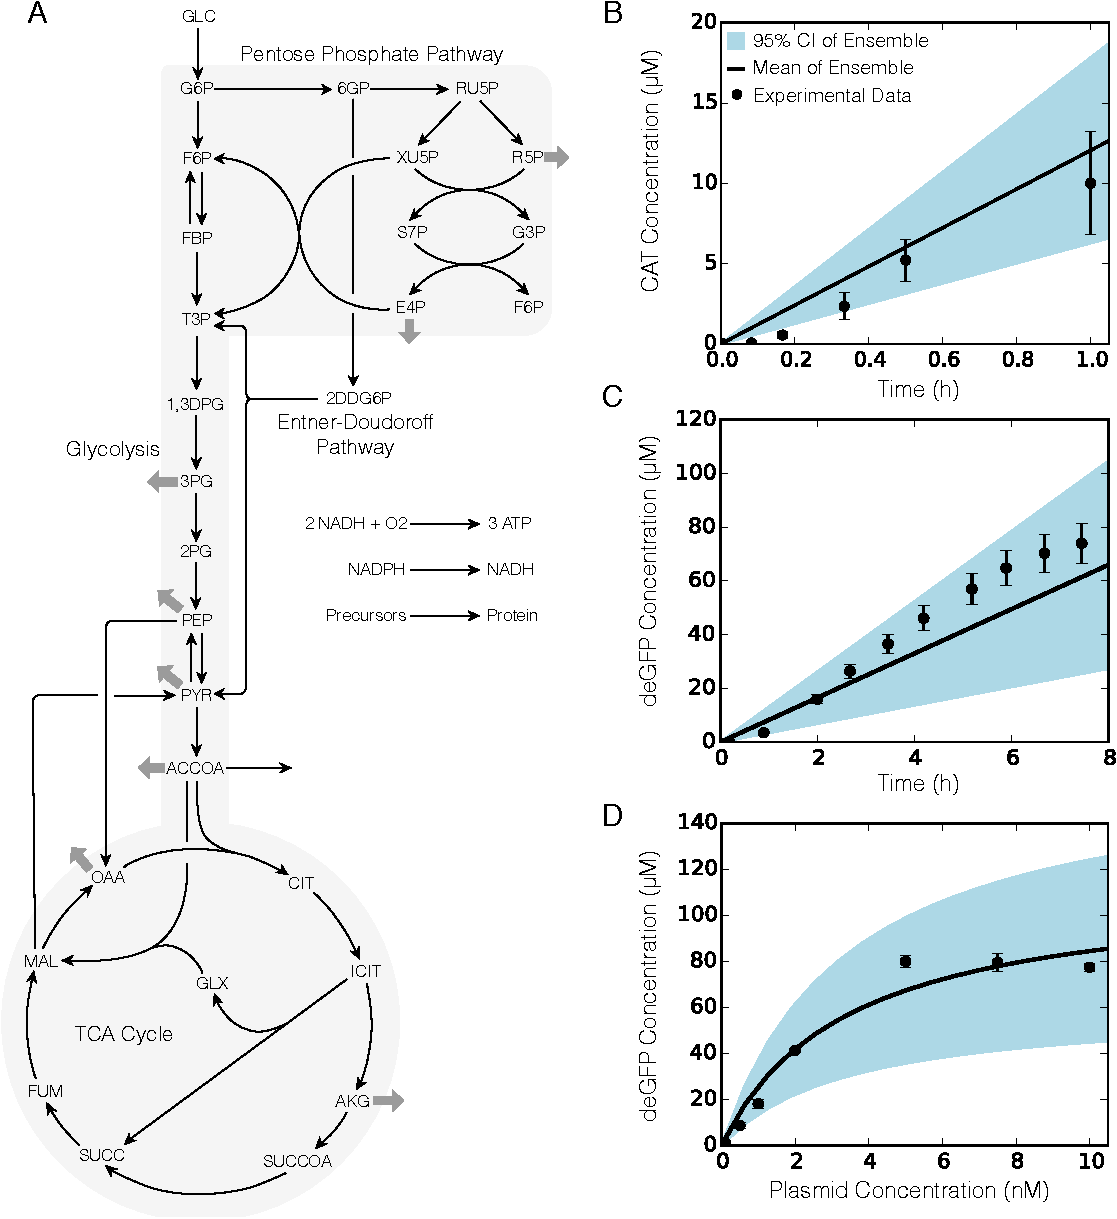
\includegraphics[width=1.00\textwidth]{./figs/Fig-1-Network-Validation-Simulations.pdf}
\caption{Sequence specific flux balance analysis.
A. Schematic of the core metabolic network describing glycolysis, pentose phosphate pathway, the TCA cycle and the Entner-Doudoroff pathway. Thick gray arrows indicate withdrawal of precursors for amino acid synthesis.
B. CAT production under a T7 promoter in CFPS \textit{E.~coli} extract for 1 h using glucose as a carbon and energy source. Error bars denote the standard deviation of experimental measurements.
C. deGFP production under a P70 promoter in TXTL 2.0 \textit{E.~coli} extract for 8 h using glucose as a carbon and energy source. Error bars denote a 10\% coefficient of variation.
D. Predicted versus measured deGFP concentration as a function of plasmid concentration in TXTL 2.0.
The blue region denotes the 95\% CI over an ensemble of N = 100 sets, the black line denotes the mean of the ensemble, and dots denote experimental measurements.}
\label{fig:network}
\end{figure}

\clearpage

\begin{figure}[t!]
\centering
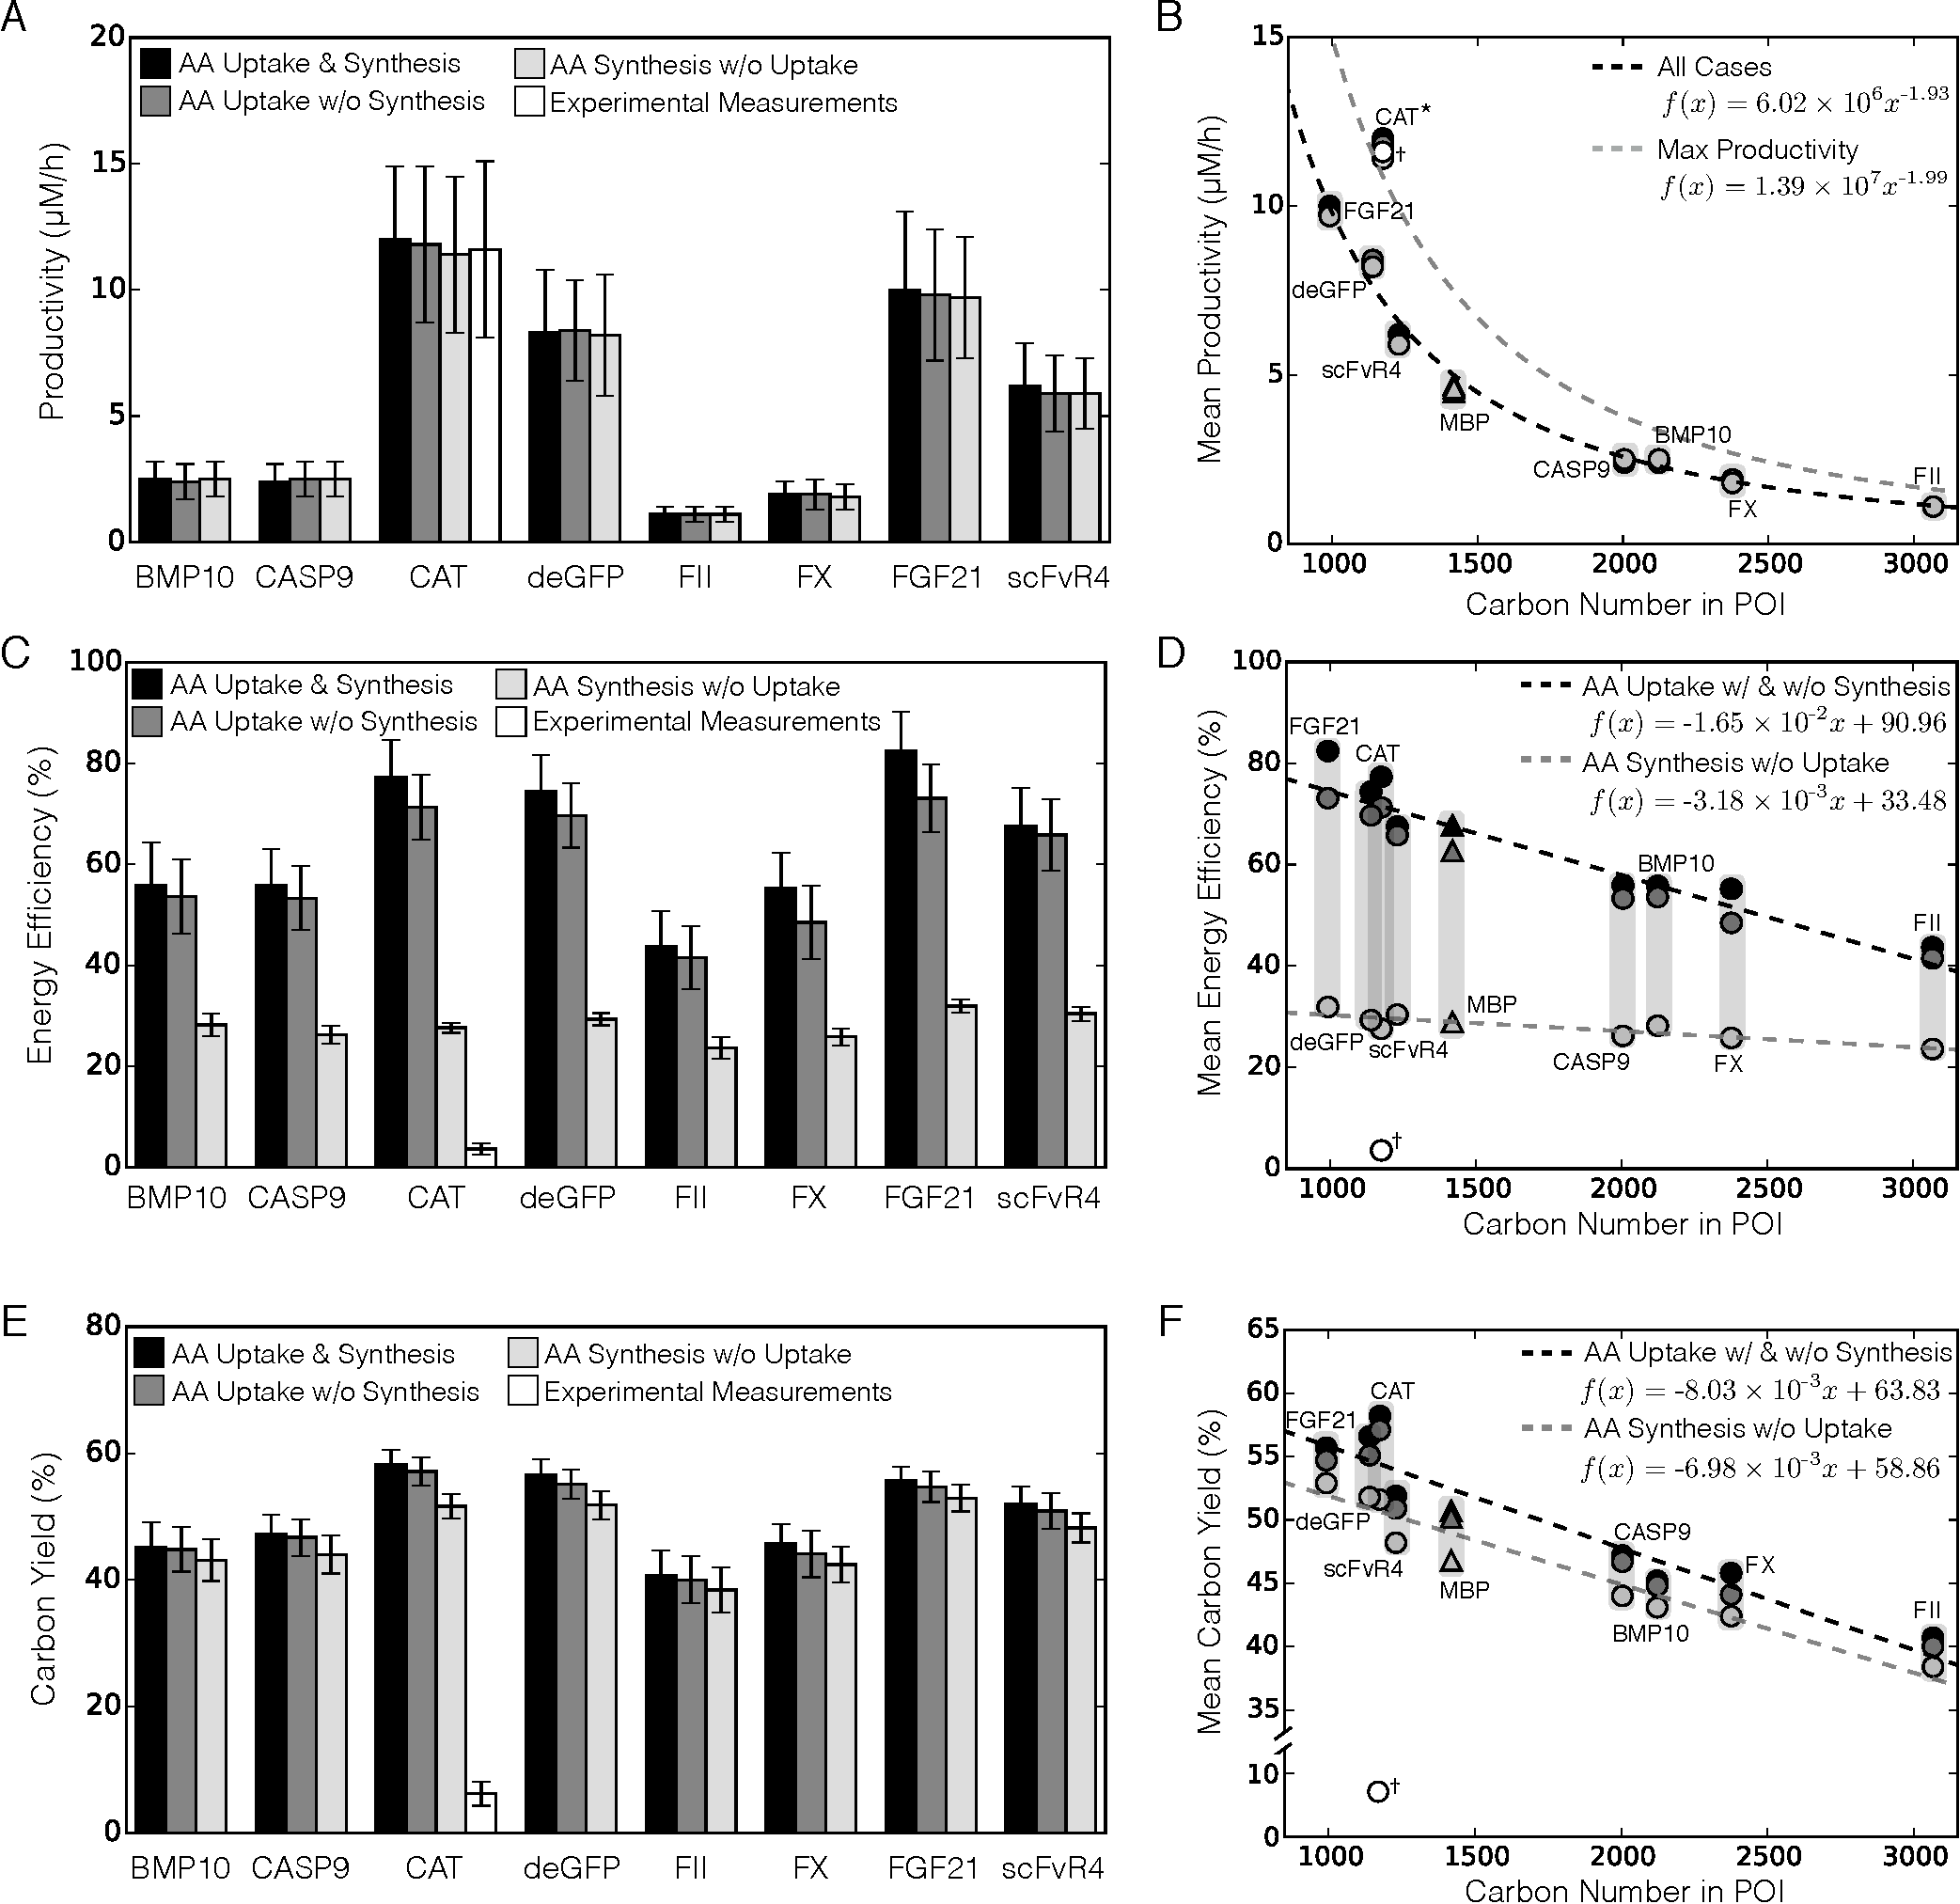
\includegraphics[width=1.00\textwidth]{./figs/Fig-2-Performance.pdf}
%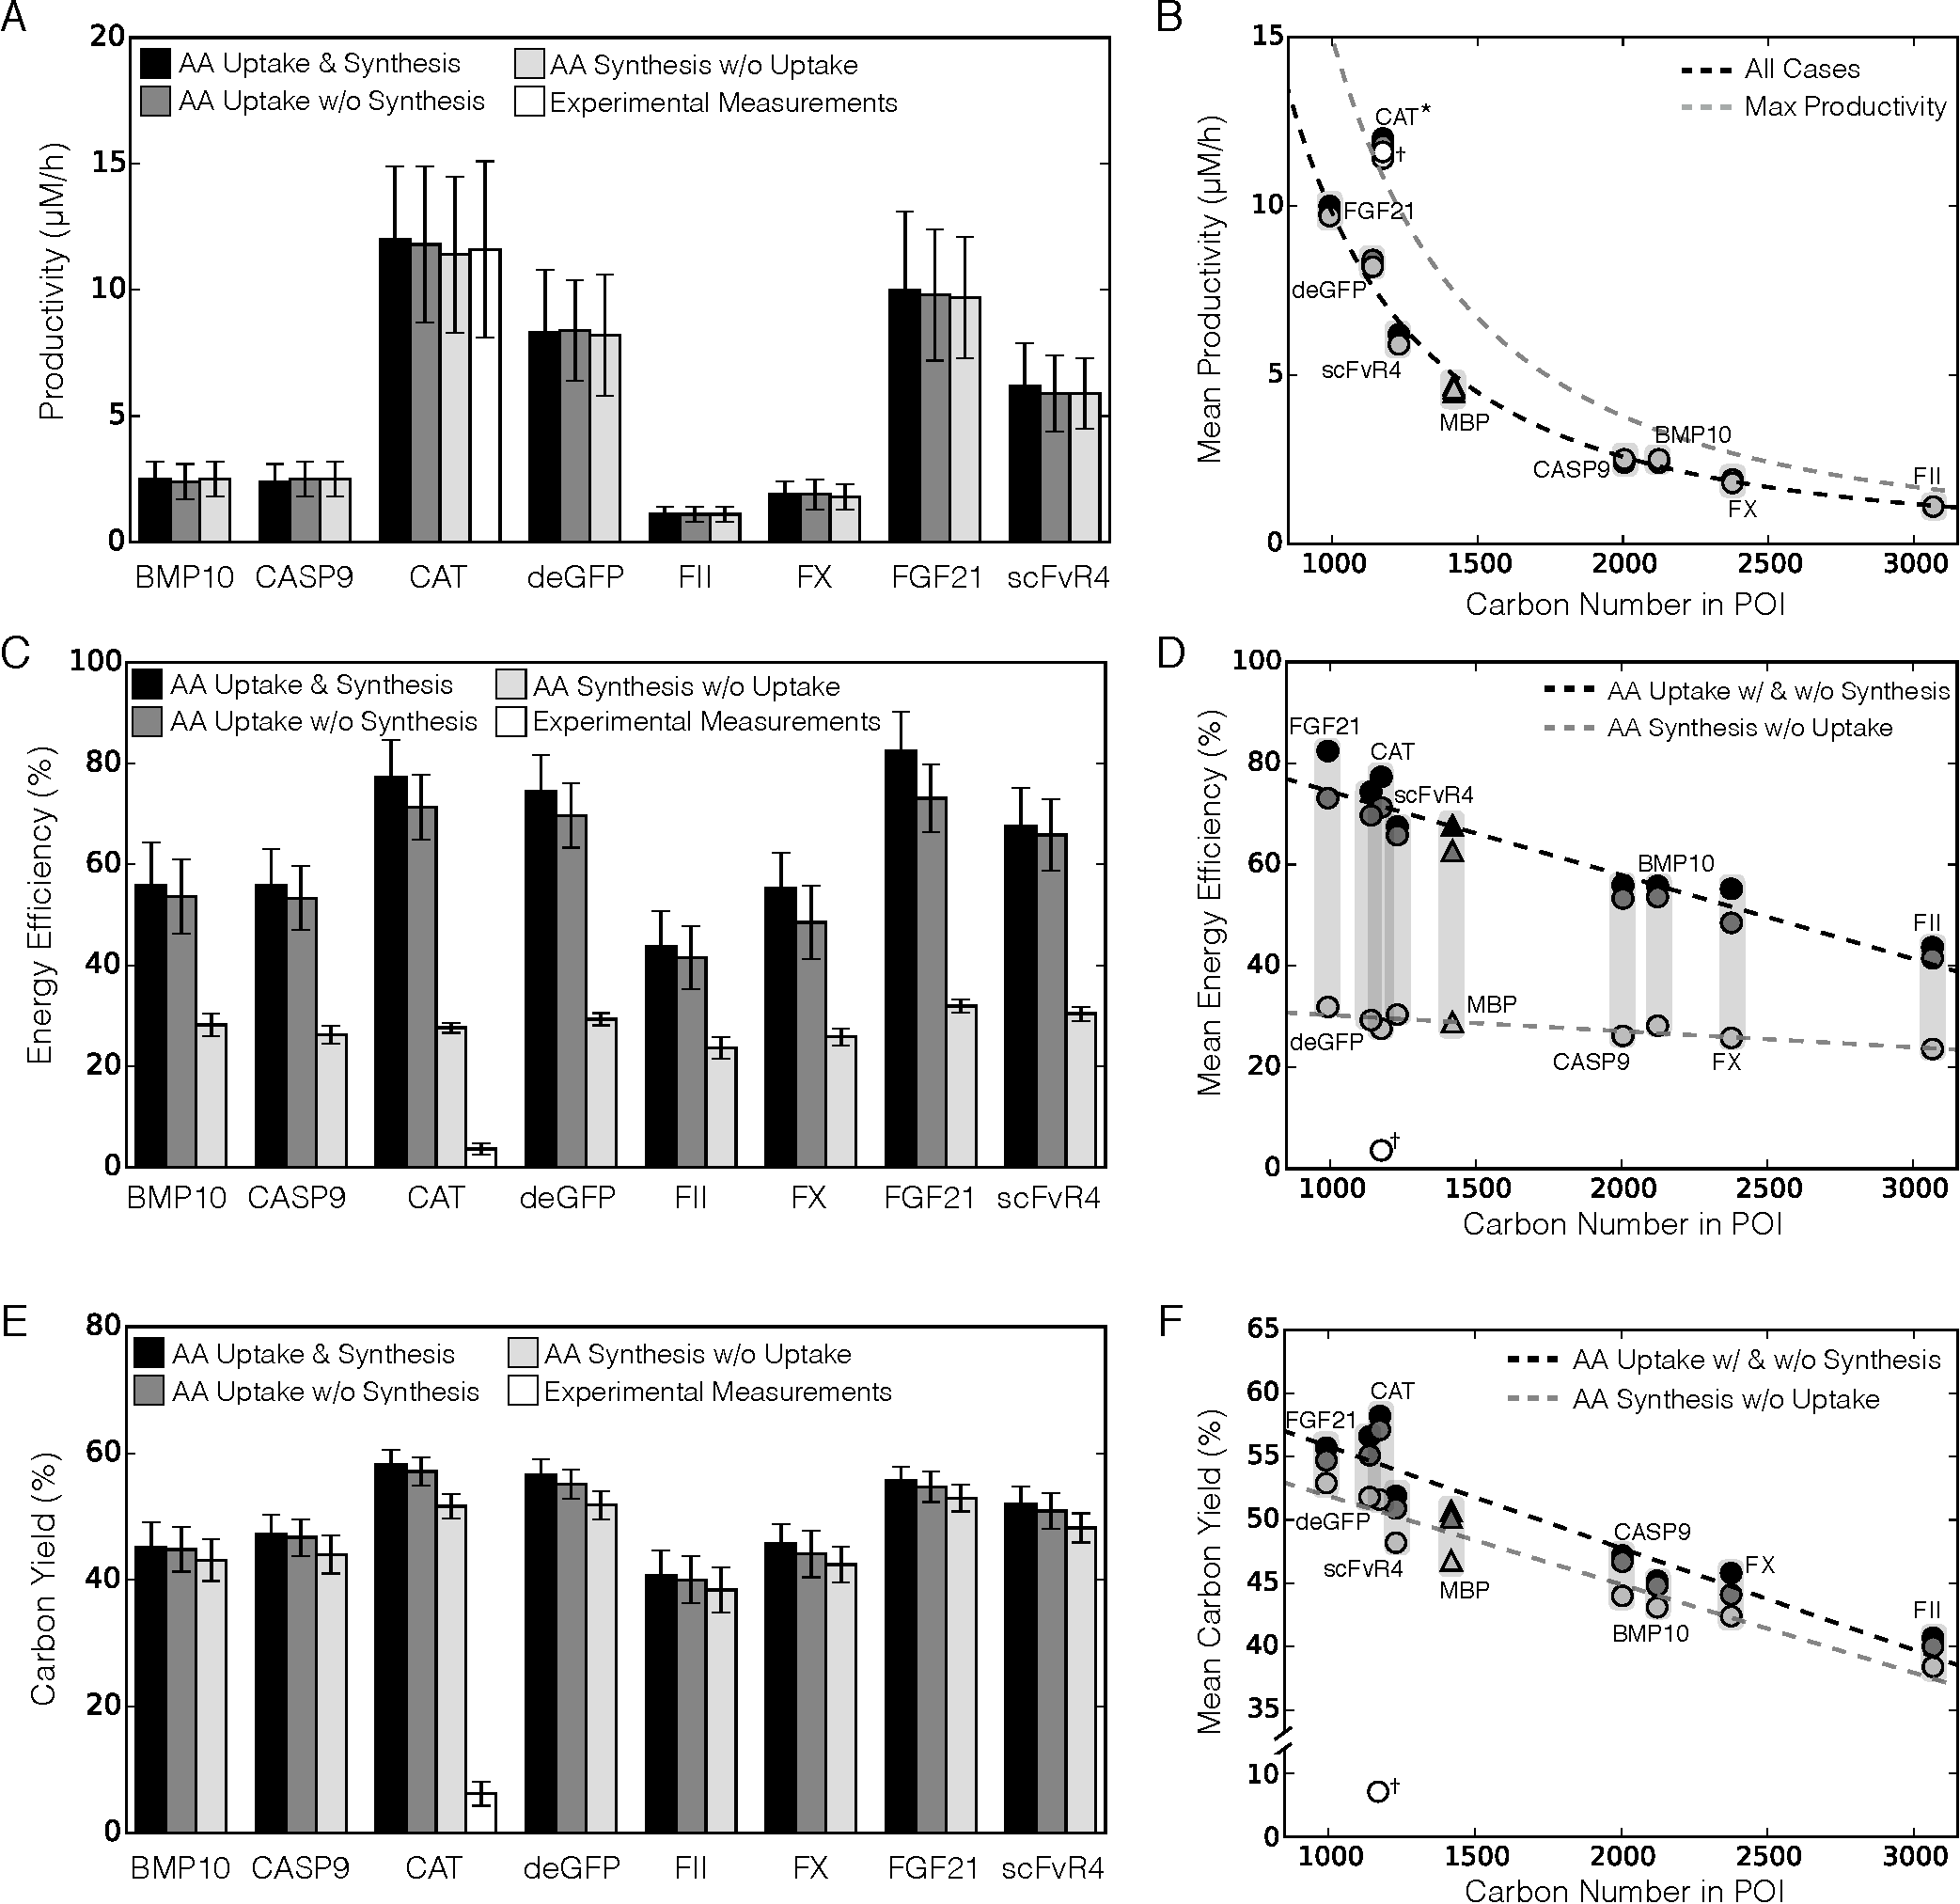
\includegraphics[width=1.00\textwidth]{./figs/Fig-2-Performance-Predicted.pdf}
\caption{The CFPS performance for eight model proteins with and without amino acid supplementation.
A. Mean CFPS productivity for a panel of model proteins with and without amino acid supplementation.
B. Mean CFPS productivity versus carbon number for a panel of model proteins with and without amino acid supplementation.
Trendline (black dotted line) was calculated across all cases for a P70a promoter (R\textsuperscript{2} = 0.99) and maximum productivity trendline assumed $u\left(\kappa\right)$ = 1 (grey dotted line; R\textsuperscript{2} = 0.99).
C. Mean CFPS energy efficiency for a panel of model proteins with and without amino acid supplementation.
D. Mean CFPS energy efficiency versus carbon number for a panel of model proteins with and without amino acid supplementation.
Trendline for cases with amino acids (black dotted line) and trendline for without amino acids (grey dotted line; R\textsuperscript{2} = 0.65).
E. Mean CFPS carbon yield for a panel of model proteins with and without amino acid supplementation.
F. Mean CFPS carbon yield versus carbon number.
Trendline for cases with amino acids (black dotted line; R\textsuperscript{2} = 0.95) and trendline for without amino acids (grey dotted line; R\textsuperscript{2} = 0.90).
Error bars: 95\% CI calculated by sampling;
asterisk: protein excluded from trendline;
dagger: constrained by experimental measurements and excluded from trendline;
triangles: first principle prediction and excluded from formulating trendline.}
\label{fig:Prof}
\end{figure}

\clearpage

\begin{figure}[t!]
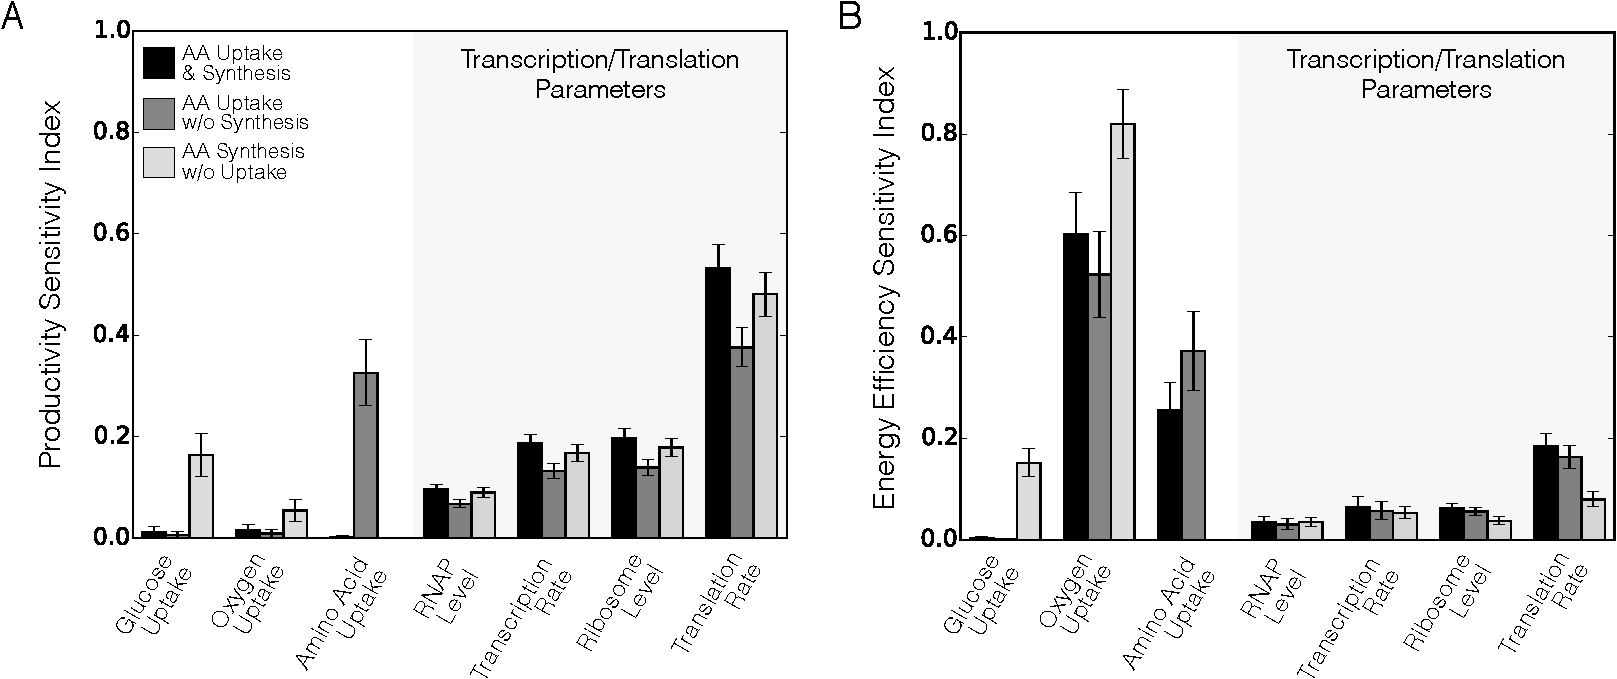
\includegraphics[width=1.00\textwidth]{./figs/Fig-3-Sensitivity-Analysis.pdf}
\caption{Total order sensitivity analysis of the cell free production of CAT.
A. Total order sensitivity of the optimal CAT productivity with respect to metabolic and transcription/translation parameters.
B. Total order sensitivity of the optimal CAT energy efficiency.
Metabolic and transcription/translation parameters were varied for amino acid supplementation and synthesis (black),
amino acid supplementation without synthesis (dark grey) and amino acid synthesis without supplementation (light gray).
Error bars represent the 95\% CI of the total order sensitivity index.}
\label{fig:SI}
\end{figure}

\clearpage

\begin{figure}[t!]
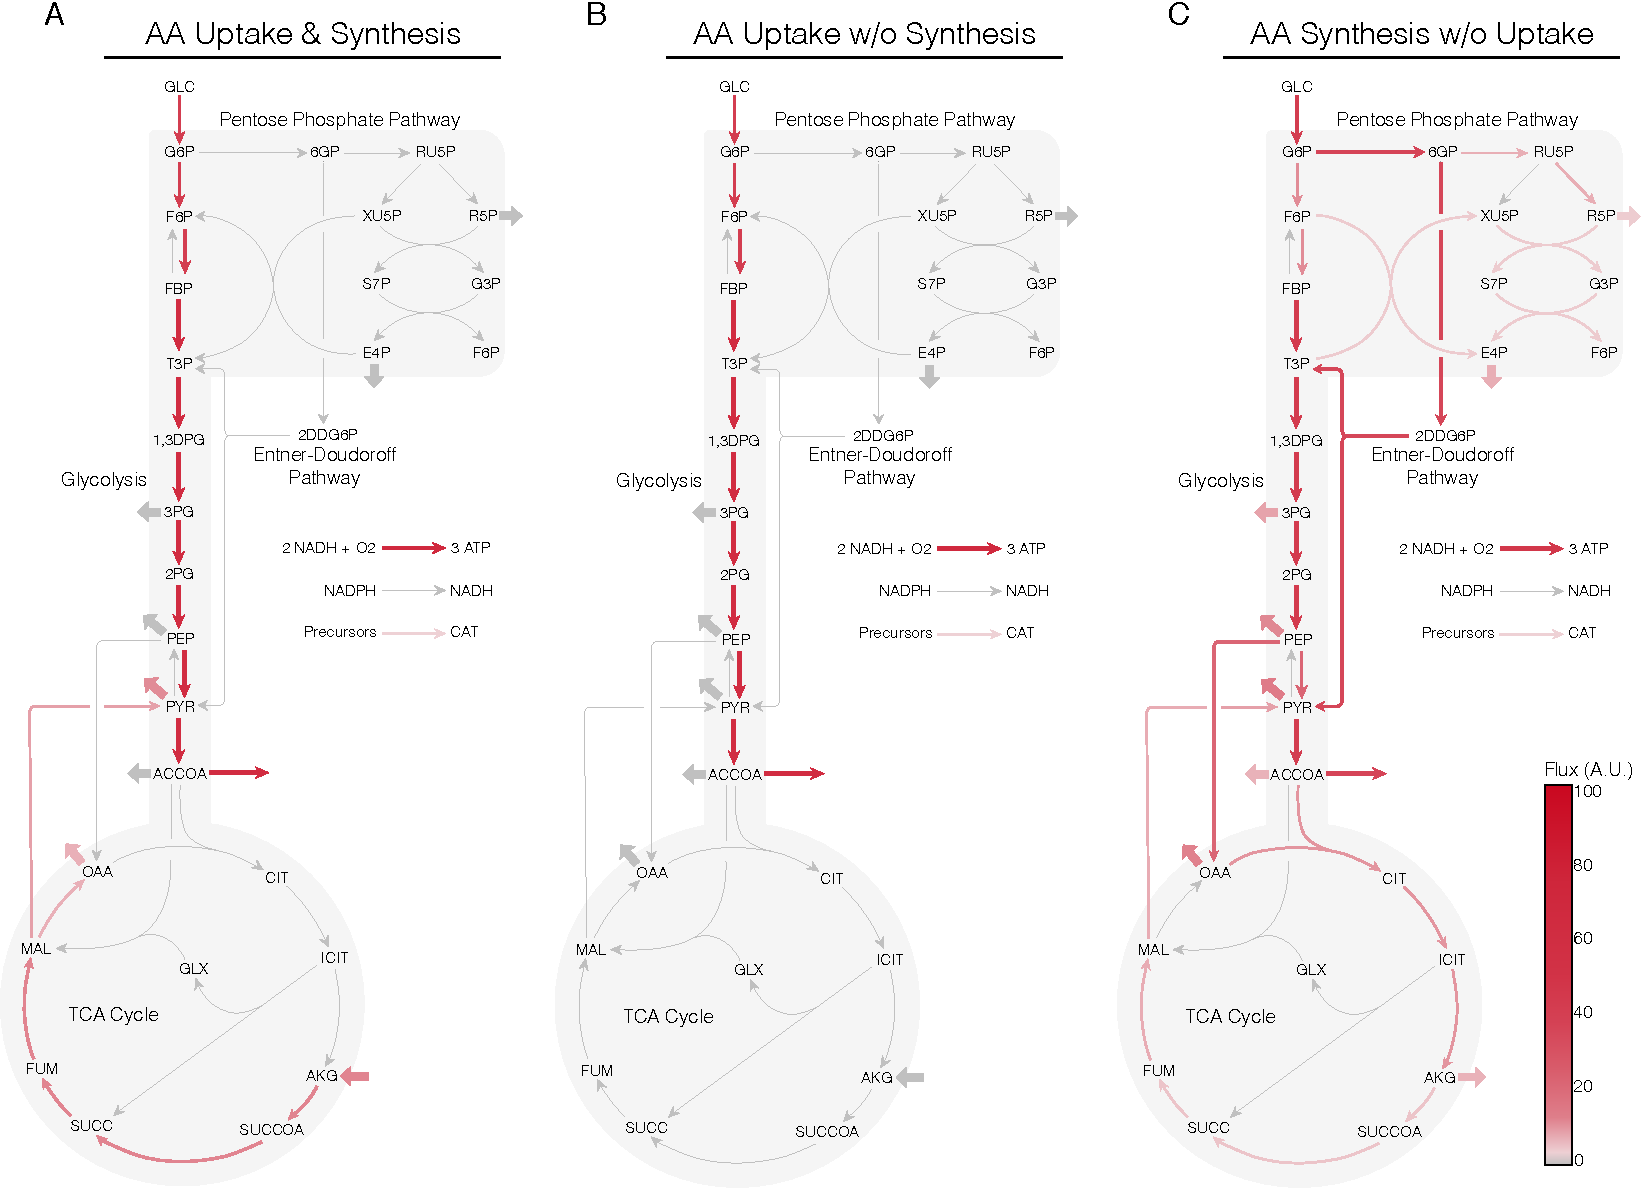
\includegraphics[width=1.00\textwidth]{./figs/Fig-5-FluxDistribition-Optimal.pdf}
\caption{Optimal metabolic flux distribution for CAT production.
A. Optimal flux distribution in the presence of amino acid supplementation and \textit{de~novo} synthesis.
B. Optimal flux distribution in the presence of amino acid supplementation without \textit{de~novo} synthesis.
C. Optimal flux distribution with \textit{de~novo} amino acid synthesis in the absence of supplementation.
Mean flux across the ensemble (N = 100), normalized to glucose uptake flux. Thick arrows indicate flux to or from amino acid biosynthesis pathways.}
\label{fig:flux}
\end{figure}

\clearpage

\begin{figure}[t!]
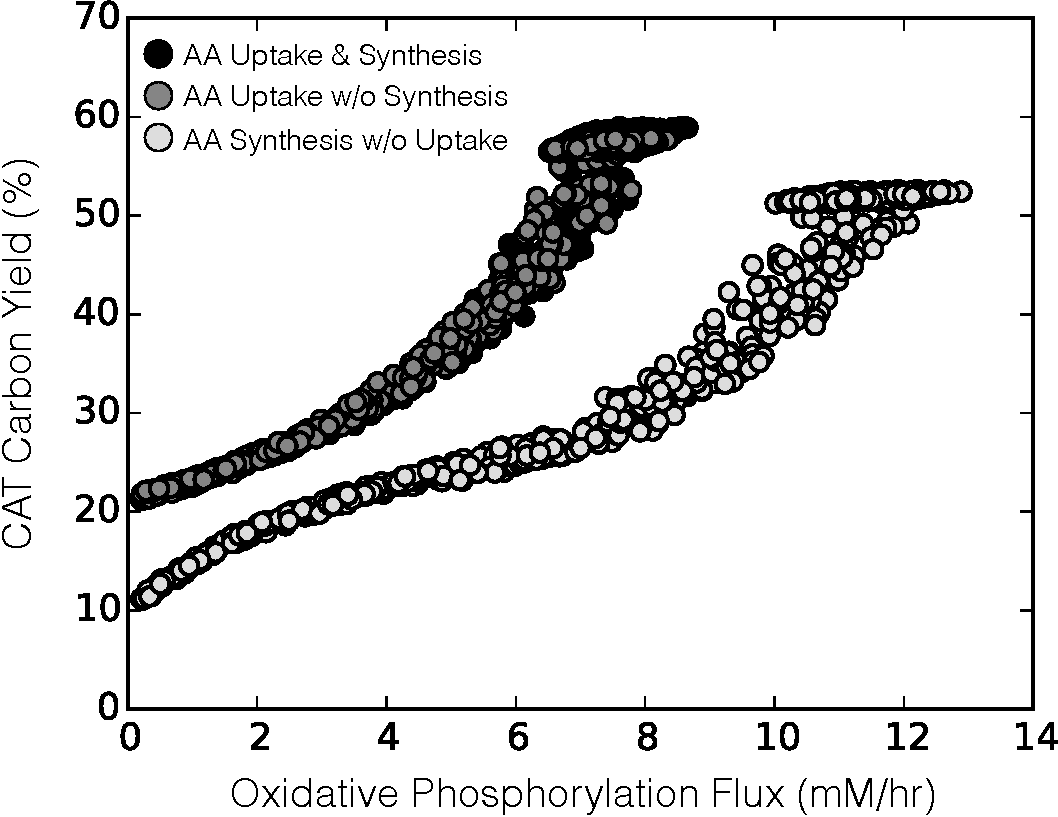
\includegraphics[width=0.7\textwidth]{./figs/Fig-4-OxyPhox-versus-Carbon-Yield.pdf}
\caption{Optimal CAT carbon yield versus oxidative phosphorylation flux calculated across an ensemble (N = 1000) flux balance solutions (points).
Carbon yield versus oxidative phosphorylation flux for amino acid supplementation and \textit{de~novo} synthesis (black),
amino acid supplementation without \textit{de~novo} synthesis (dark grey),
and \textit{de~novo} amino acid synthesis without supplementation (light gray).}
\label{fig:oxphos_yield}
\end{figure}


\clearpage

\begin{figure}[t!]
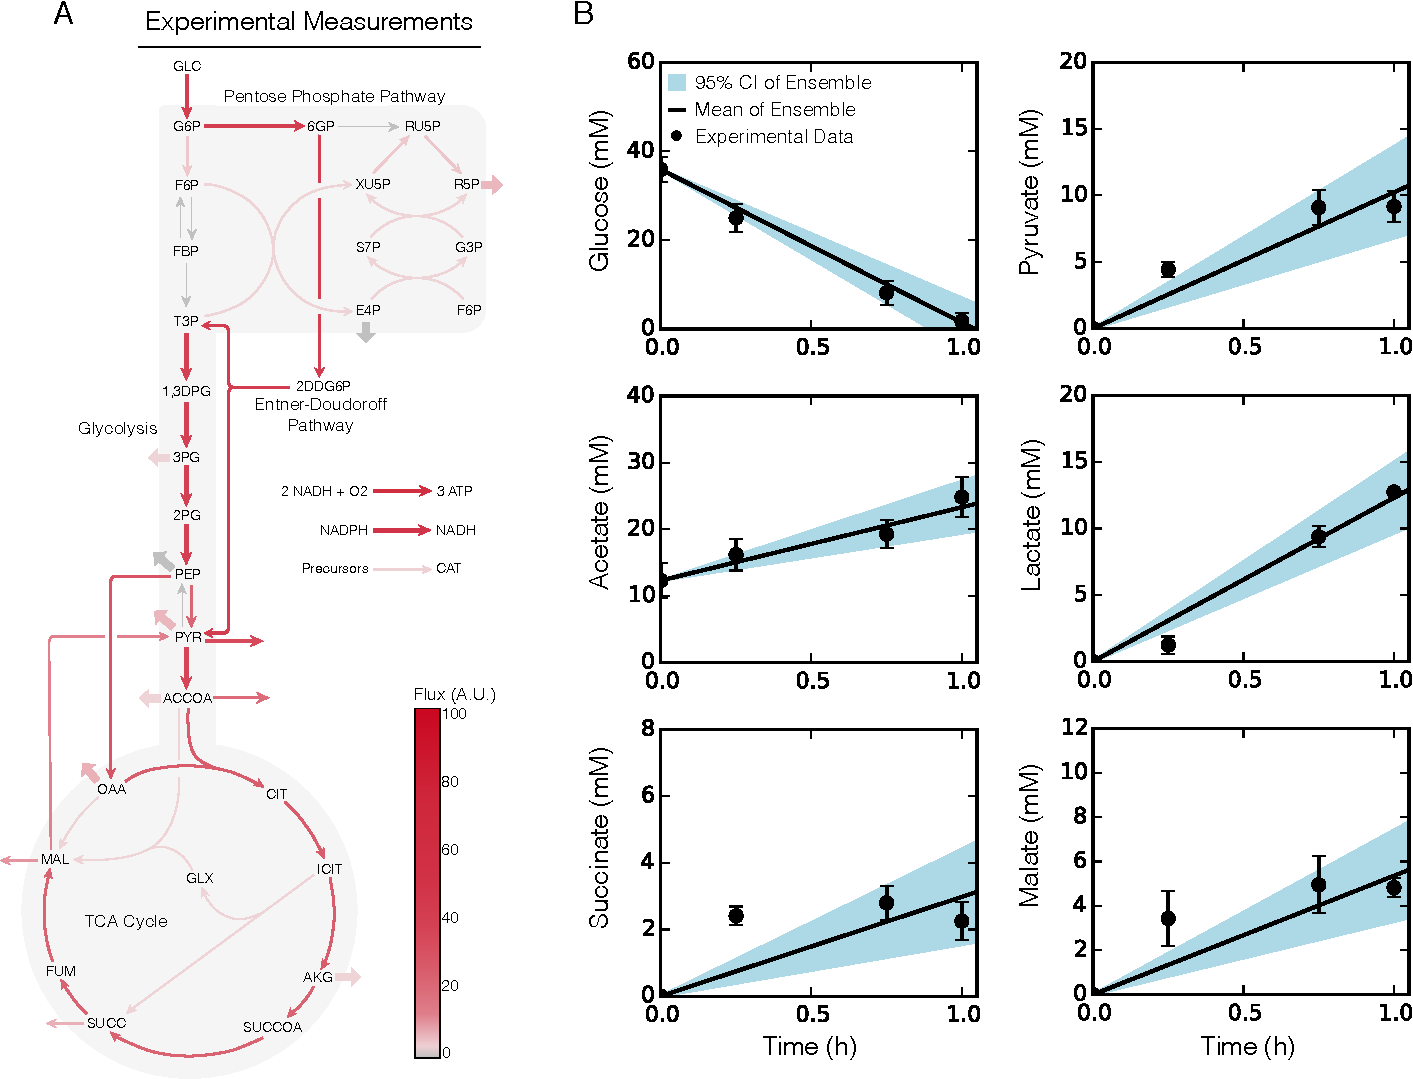
\includegraphics[width=1.00\textwidth]{./figs/Fig-6-FluxDistribition-Experimental.pdf}
\caption{Experimentally constraint based simulation of CAT production.
A. Metabolic flux distribution for CAT production in the presence of experimental constraints for glucose, organic acid and amino acid consumption and production rates.
Mean flux across the ensemble, normalized to glucose uptake flux. Thick arrows indicate flux to or from amino acids.
B. Central carbon metabolite measurements versus simulations over a 1 hour time course.
The blue region denotes the 95\% CI over an ensemble of N = 100 sets, the black line denotes the mean of the ensemble, and dots denote experimental measurements.}
\label{fig:flux_exp}
\end{figure}

\clearpage

\begin{figure}[t!]
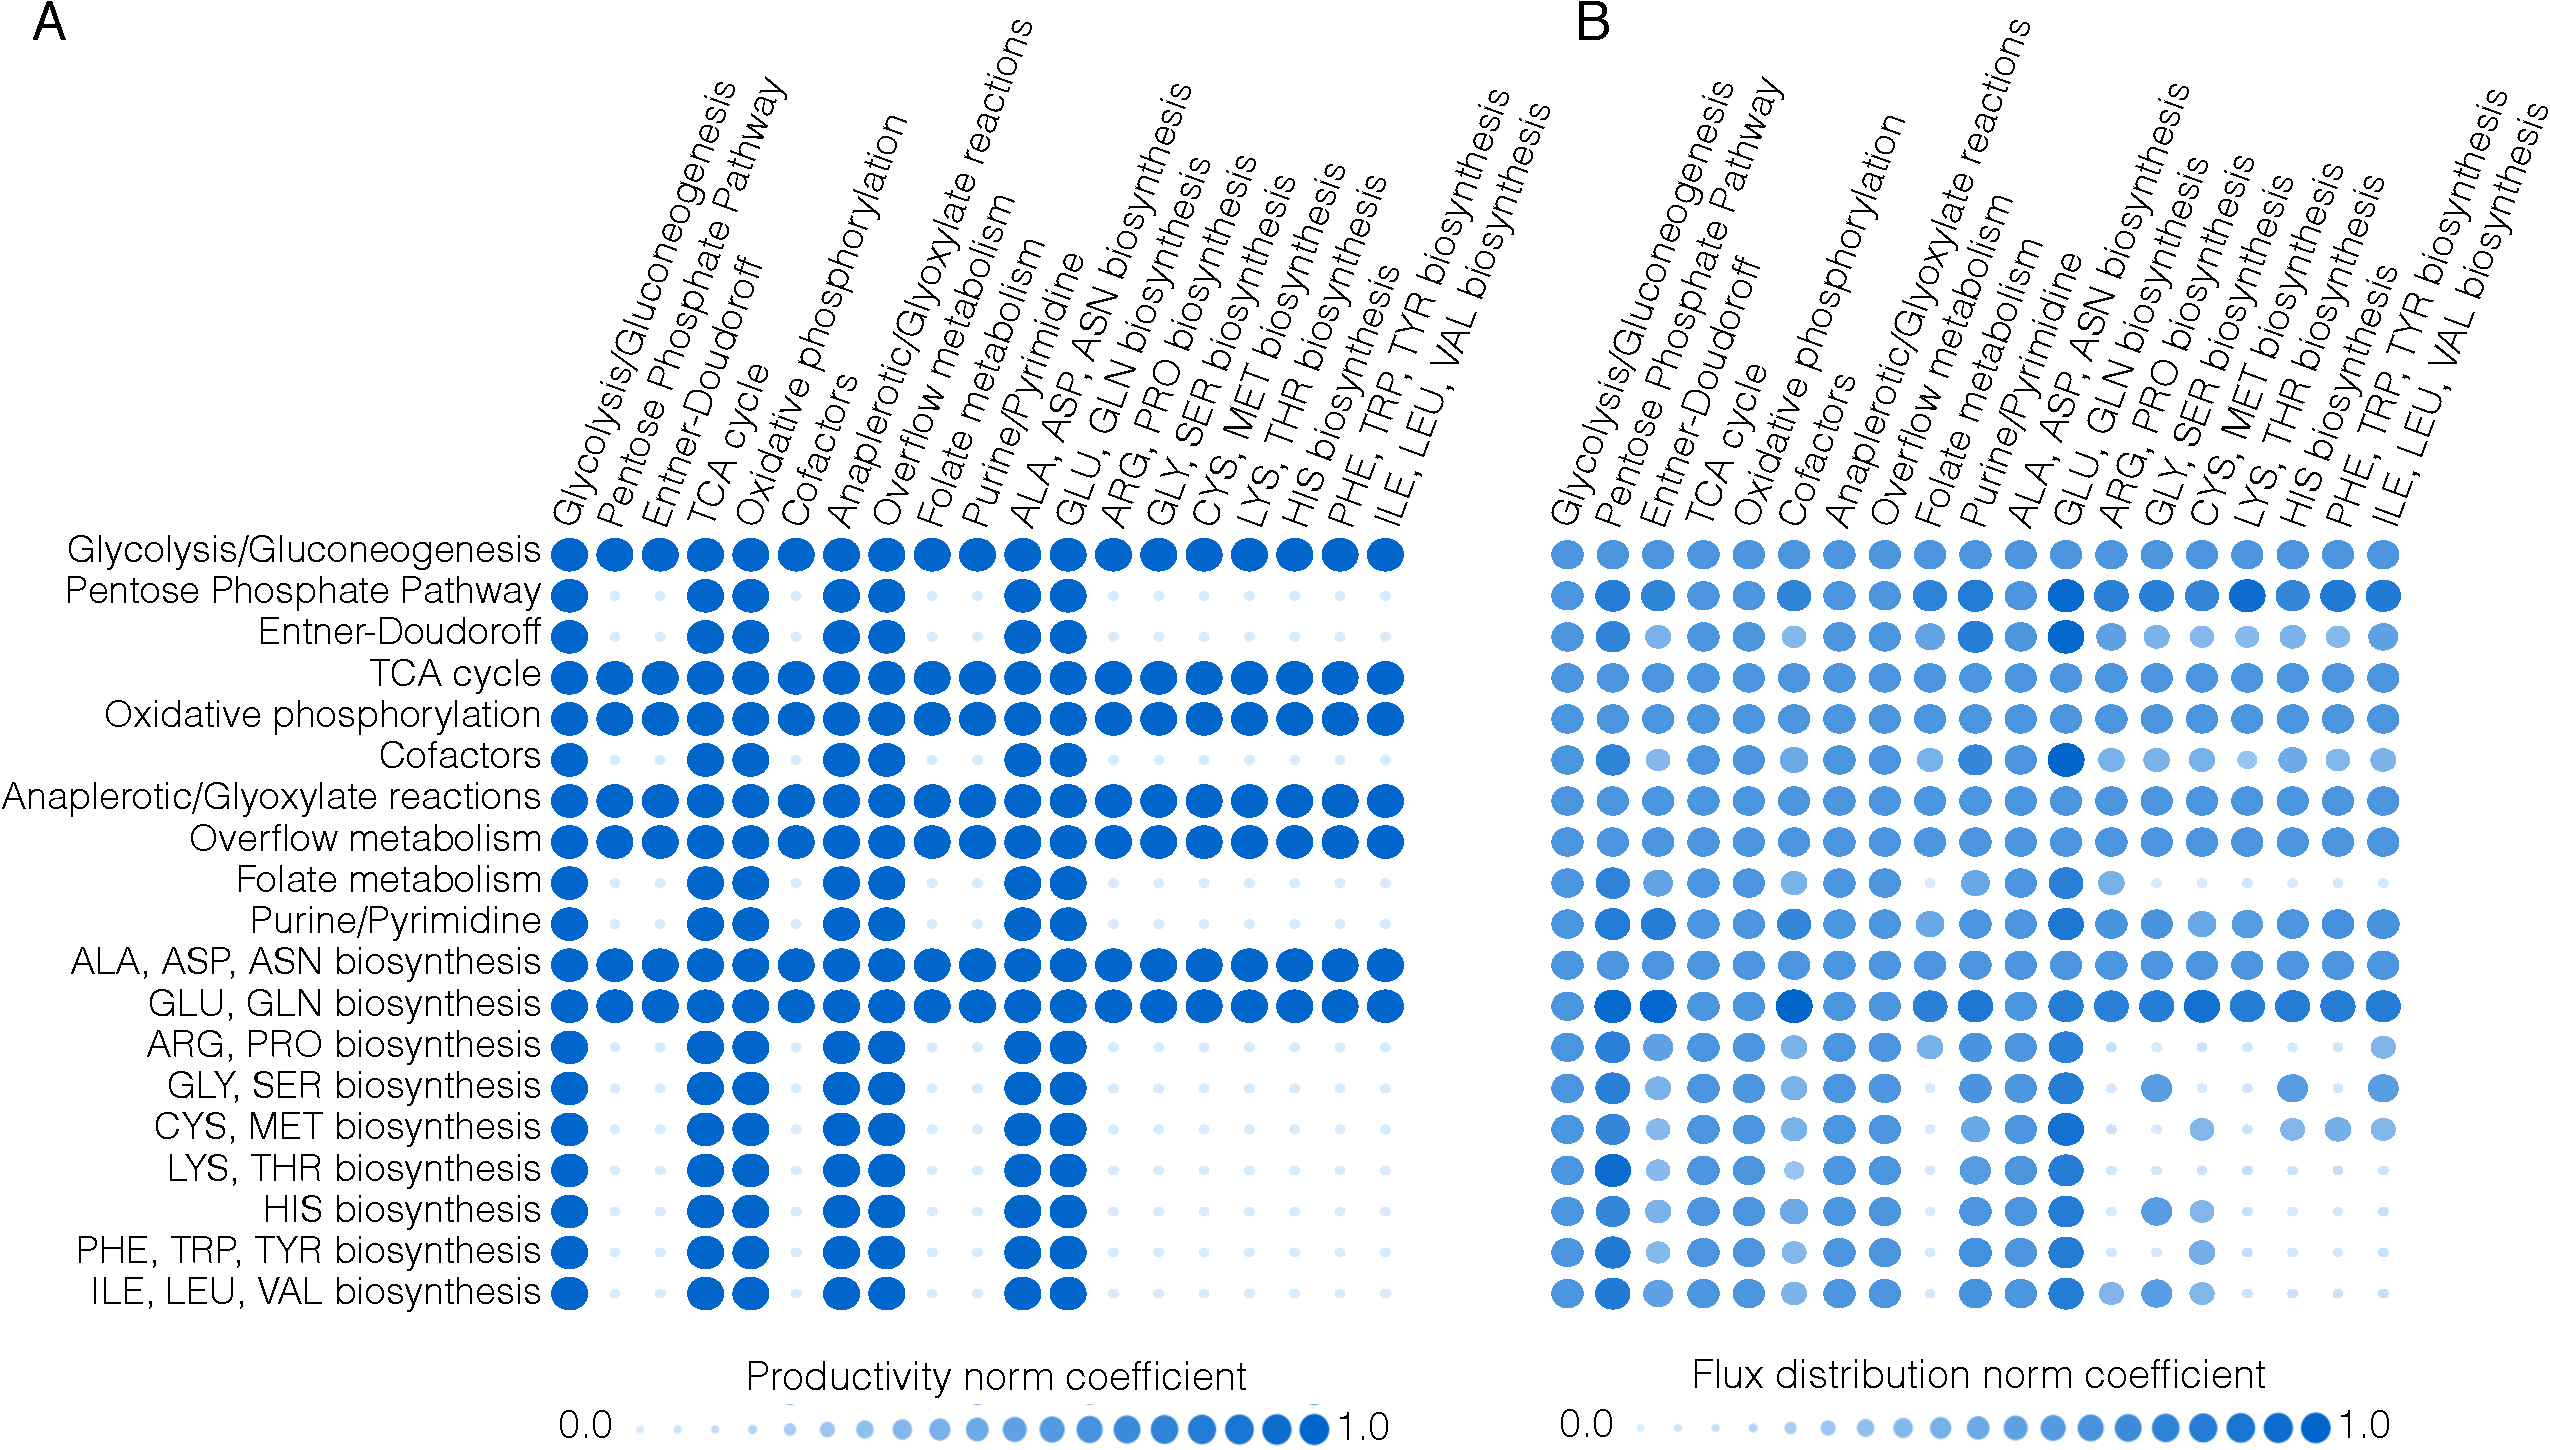
\includegraphics[width=1.0\textwidth]{./figs/Fig-7-FluxDistribution-Analysis.pdf}
\caption{Pairwise knockouts of reaction subgroups in the cell-free network.
A. Difference in the CAT productivity in the presence of reaction knockouts compared with no knockouts for experimentally constrained CAT production.
B. Difference in the optimal flux distribution in the presence of reaction knockouts compared with no knockouts for experimentally constrained CAT production.
The difference between perturbed and wild-type productivity and flux distributions was quantified by the $l^{2}$ norm, and then normalized so the maximum change was 1.0.
Red boxes indicate potential alternative optimal flux distributions.}
\label{fig:norm}
\end{figure}

\clearpage

\bibliography{References_v1}

\end{document}
\grid
